\documentclass[12pt,a4paper]{report}

%% ── Encodage & langue ──────────────────────────────────────────────────────
\usepackage[utf8]{inputenc}
\usepackage[T1]{fontenc}
\usepackage[provide=*,french,shorthands=off]{babel}
\usepackage{lmodern}
\usepackage{microtype}

%% ── Mise en page ───────────────────────────────────────────────────────────
\usepackage[top=2.5cm, bottom=2.5cm, left=3cm, right=2.5cm]{geometry}
\usepackage{setspace}
\usepackage{parskip}
\onehalfspacing

%% ── En-têtes et pieds de page ──────────────────────────────────────────────
\usepackage{fancyhdr}
\pagestyle{fancy}
\fancyhf{}
\fancyhead[L]{\small\textit{ABIS -- AI Blockchain Immune System}}
\fancyhead[R]{\small\textit{Rapport de Projet}}
\fancyfoot[C]{\thepage}
\renewcommand{\headrulewidth}{0.4pt}
\renewcommand{\footrulewidth}{0.4pt}

%% ── Titres de chapitres ────────────────────────────────────────────────────
\usepackage{titlesec}
\titleformat{\chapter}[display]
  {\normalfont\huge\bfseries\color{deepblue}}
  {\chaptertitlename\ \thechapter}{20pt}{\Huge}
\titlespacing*{\chapter}{0pt}{30pt}{20pt}

%% ── Couleurs ────────────────────────────────────────────────────────────────
\usepackage[dvipsnames,table]{xcolor}
\definecolor{deepblue}{RGB}{0,51,102}
\definecolor{medblue}{RGB}{0,102,204}
\definecolor{lightblue}{RGB}{220,235,250}
\definecolor{deepgreen}{RGB}{0,100,0}
\definecolor{lightgreen}{RGB}{220,245,220}
\definecolor{deepred}{RGB}{160,0,0}
\definecolor{lightyellow}{RGB}{255,253,220}
\definecolor{codebg}{RGB}{248,248,248}
\definecolor{codeframe}{RGB}{200,200,200}
\definecolor{warnorange}{RGB}{230,100,0}

%% ── Boîtes colorées ─────────────────────────────────────────────────────────
\usepackage[most]{tcolorbox}
\tcbuselibrary{listings,breakable,skins}

\newtcolorbox{infobox}[1][]{
  colback=lightblue, colframe=medblue, fonttitle=\bfseries,
  title=#1, breakable, boxrule=0.5pt, arc=3pt
}
\newtcolorbox{warningbox}[1][]{
  colback=lightyellow, colframe=warnorange, fonttitle=\bfseries,
  title=#1, breakable, boxrule=0.5pt, arc=3pt
}
\newtcolorbox{successbox}[1][]{
  colback=lightgreen, colframe=deepgreen, fonttitle=\bfseries,
  title=#1, breakable, boxrule=0.5pt, arc=3pt
}
\newtcolorbox{codebox}[1][]{
  colback=codebg, colframe=codeframe, fonttitle=\bfseries\small,
  title=#1, breakable, boxrule=0.5pt, arc=3pt
}

%% ── Listings (code source) ──────────────────────────────────────────────────
\usepackage{listings}
\lstset{
  backgroundcolor=\color{codebg},
  basicstyle=\ttfamily\small,
  breaklines=true,
  breakatwhitespace=false,
  captionpos=b,
  commentstyle=\color{deepgreen}\itshape,
  frame=single,
  framerule=0.5pt,
  keepspaces=true,
  keywordstyle=\color{medblue}\bfseries,
  numbers=left,
  numbersep=8pt,
  numberstyle=\tiny\color{gray},
  rulecolor=\color{codeframe},
  showspaces=false,
  showstringspaces=false,
  showtabs=false,
  stepnumber=1,
  stringstyle=\color{deepred},
  tabsize=2,
  xleftmargin=15pt,
}
\lstdefinelanguage{Solidity}{
  keywords={pragma, solidity, contract, function, address, uint256, uint8,
    bool, mapping, struct, event, modifier, require, emit, returns,
    public, private, external, internal, view, pure, payable, override,
    virtual, is, memory, storage, calldata, if, else, for, while, return,
    constructor, indexed, bytes, string, bytes32, uint},
  sensitive=true,
  comment=[l]{//},
  morecomment=[s]{/*}{*/},
  morestring=[b]",
}
\lstdefinelanguage{Python}{
  keywords={def, class, import, from, return, if, elif, else, for, while,
    in, not, and, or, True, False, None, try, except, with, as, pass,
    break, continue, lambda, yield, async, await, global, nonlocal,
    del, raise, finally, assert},
  sensitive=true,
  comment=[l]{\#},
  morestring=[b]",
  morestring=[b]',
}

%% ── Tableaux ────────────────────────────────────────────────────────────────
\usepackage{booktabs}
\usepackage{multirow}
\usepackage{tabularx}
\usepackage{array}
\newcolumntype{L}[1]{>{\raggedright\arraybackslash}p{#1}}
\newcolumntype{C}[1]{>{\centering\arraybackslash}p{#1}}
\newcolumntype{R}[1]{>{\raggedleft\arraybackslash}p{#1}}

%% ── Figures ─────────────────────────────────────────────────────────────────
\usepackage{graphicx}
\usepackage{caption}
\usepackage{subcaption}
\usepackage{float}

%% ── TikZ (diagrammes) ───────────────────────────────────────────────────────
\usepackage{tikz}
\usetikzlibrary{shapes.geometric, arrows.meta, positioning, fit, backgrounds,
  decorations.pathreplacing, calc}

%% ── Énumérations ─────────────────────────────────────────────────────────────
\usepackage{enumitem}
\setlist[itemize]{leftmargin=*, nosep}
\setlist[enumerate]{leftmargin=*, nosep}

%% ── Cadres ───────────────────────────────────────────────────────────────────
\usepackage[framemethod=default]{mdframed}

%% ── Citations ─────────────────────────────────────────────────────────────────
\usepackage{csquotes}

%% ── Pifont (symboles) ────────────────────────────────────────────────────────
\usepackage{pifont}
\newcommand{\cmark}{\ding{51}}
\newcommand{\xmark}{\ding{55}}
\newcommand{\arrow}{\ding{220}}

%% ── Hyperliens ────────────────────────────────────────────────────────────────
\usepackage[hidelinks,
  pdfauthor={Yassine Allani, Maryem El Bekri, Abderrahmen Ben Khlifa},
  pdftitle={ABIS -- AI Blockchain Immune System -- Rapport de Projet},
  pdfsubject={Système de sécurité DeFi par intelligence artificielle},
  pdfkeywords={blockchain, IA, sécurité, DeFi, isolation forest, random forest}
]{hyperref}

%% ── Commandes utilitaires ─────────────────────────────────────────────────────
\newcommand{\abis}{\textbf{ABIS}}
\newcommand{\code}[1]{\texttt{#1}}
\newcommand{\term}[1]{\textit{#1}}

%% ═════════════════════════════════════════════════════════════════════════════
\begin{document}
\pagenumbering{roman}

%% ── PAGE DE COUVERTURE ────────────────────────────────────────────────────────
\begin{titlepage}
\centering
\thispagestyle{empty}

% Logo

\includegraphics[width=4cm]{tek_up_logo.png}\\[0.5cm]

% Filet supérieur
{\color{deepblue}\rule{\linewidth}{2pt}}\\[0.3cm]

% Université
{\large\bfseries\color{deepblue} Université Privée de Tunis --- Tek-UP}\\[0.2cm]
{\large Département Informatique}\\[0.2cm]
{\normalsize Année Académique 2025--2026}\\[0.5cm]

% Filet
{\color{deepblue}\rule{\linewidth}{0.5pt}}\\[0.8cm]

% Type de rapport
\begin{tcolorbox}[colback=deepblue, coltext=white, boxrule=0pt, arc=5pt,
    halign=center, width=0.8\linewidth]
  {\Large\bfseries Rapport de Projet de Fin d'Études}
\end{tcolorbox}
\vspace{0.6cm}

% Titre principal
{\Huge\bfseries\color{deepblue} ABIS}\\[0.3cm]
{\Large\bfseries\color{medblue} AI Blockchain Immune System}\\[0.3cm]
{\large\color{deepblue}\itshape Système de Détection et de Réponse aux Attaques\\
dans les Protocoles DeFi par Intelligence Artificielle}\\[1cm]

% Filet
{\color{deepblue}\rule{0.6\linewidth}{0.5pt}}\\[1cm]

% Auteurs
{\large\bfseries Réalisé par :}\\[0.4cm]
\begin{tcolorbox}[colback=lightblue, colframe=medblue, boxrule=0.5pt,
    arc=3pt, width=0.65\linewidth, halign=center]
\begin{tabular}{c}
  {\large \textbf{Yassine Allani}}\\[0.2cm]
  {\large \textbf{Maryem El Bekri}}\\[0.2cm]
  {\large \textbf{Abderrahmen Ben Khlifa}}
\end{tabular}
\end{tcolorbox}

\vfill

% Bas de page
{\color{deepblue}\rule{\linewidth}{0.5pt}}\\[0.3cm]
{\normalsize Projet soumis au jury de l'Université Tek-UP --- Juin 2026}

\end{titlepage}

%% ── PAGE DÉDICACE ─────────────────────────────────────────────────────────────
\newpage
\thispagestyle{empty}
\vspace*{5cm}
\begin{flushright}
\begin{minipage}{0.6\linewidth}
\itshape
\textit{À nos familles, pour leur soutien indéfectible tout au long de ce parcours.}\\[0.5cm]
\textit{À nos enseignants de Tek-UP, pour leur accompagnement et leurs précieux conseils.}\\[0.5cm]
\textit{À la communauté open source, dont les travaux ont rendu ce projet possible.}
\end{minipage}
\end{flushright}

%% ── REMERCIEMENTS ─────────────────────────────────────────────────────────────
\newpage
\chapter*{Remerciements}
\addcontentsline{toc}{chapter}{Remerciements}

Nous tenons à exprimer notre profonde gratitude à toutes les personnes qui ont contribué à la réalisation de ce projet.

Nos remerciements s'adressent en premier lieu à nos encadrants et enseignants de l'Université Tek-UP, pour leur disponibilité, leurs orientations précieuses et leur engagement pédagogique tout au long de cette année académique.

Nous remercions également nos familles et nos proches pour leur soutien moral constant, leur patience et leur encouragement sans faille durant les périodes les plus intenses de ce projet.

Un remerciement particulier est adressé à la communauté scientifique et open source pour les ressources et outils mis à disposition : les équipes de développement d'Ethereum, Hardhat, scikit-learn, React et FastAPI, dont les travaux constituent le socle technologique d'ABIS.

Enfin, nous remercions les membres du jury pour le temps qu'ils consacrent à l'évaluation de ce travail et pour leur retour constructif.

%% ── RÉSUMÉ ────────────────────────────────────────────────────────────────────
\newpage
\chapter*{Résumé}
\addcontentsline{toc}{chapter}{Résumé}

La Finance Décentralisée (DeFi) connaît une croissance exponentielle depuis 2020, atteignant des milliards de dollars de valeur totale bloquée. Cependant, cette expansion s'accompagne d'une recrudescence des attaques sophistiquées : \textit{flash loans}, manipulations de prix, attaques Sybil, drainages progressifs et exploits de smart contracts. Les mécanismes de protection existants restent insuffisants face à la diversité et à la subtilité de ces menaces.

Ce rapport présente \textbf{ABIS} (\textit{AI Blockchain Immune System}), un système autonome de détection et de réponse aux attaques dans les protocoles DeFi. ABIS repose sur une architecture à trois couches interdépendantes :

\begin{itemize}
  \item \textbf{Couche Blockchain} : Cinq smart contracts Solidity déployés sur une infrastructure Hardhat, intégrant un modificateur de garde universel (\code{abisGuard}) appliqué à chaque fonction protégée, avec un système d'enforcement à quatre niveaux (WARN, BLOCK\_PROTOCOL, BLOCK, FREEZE).
  \item \textbf{Couche Intelligence Artificielle} : Un agent Python autonome combinant un \textit{IsolationForest} non supervisé (entraîné sur 170\,000 transactions normales) et un \textit{RandomForest} supervisé (150\,000 échantillons d'attaques, 48 types) via un scoring hybride. L'agent analyse trois fenêtres temporelles glissantes et intègre deux mécanismes d'amplification : détection des attaques lentes (A2) et coordination Sybil (A1).
  \item \textbf{Couche Dashboard} : Une API FastAPI avec 25+ endpoints et un tableau de bord React 19 temps réel, permettant visualisation, configuration et simulation des attaques.
\end{itemize}

Les expérimentations menées sur un nœud Ethereum local (Hardhat) avec 48 types d'attaques simulées démontrent un taux de détection supérieur à 94\%, un temps de réponse inférieur à 3 secondes, et une discrimination fiable entre comportements normaux et malveillants.

\textbf{Mots-clés :} DeFi, Blockchain Security, Isolation Forest, Random Forest, Smart Contracts, Sybil Detection, Anomaly Detection, Real-time Monitoring.

%% ── ABSTRACT (anglais) ────────────────────────────────────────────────────────
\newpage
\chapter*{Abstract}
\addcontentsline{toc}{chapter}{Abstract}

Decentralized Finance (DeFi) has experienced exponential growth since 2020, reaching billions of dollars in Total Value Locked (TVL). This expansion has been accompanied by increasingly sophisticated attacks: flash loans, price manipulation, Sybil attacks, gradual draining, and smart contract exploits. Existing protection mechanisms remain insufficient against the diversity and subtlety of these threats.

This report presents \textbf{ABIS} (\textit{AI Blockchain Immune System}), an autonomous attack detection and response system for DeFi protocols. ABIS relies on a three-layer interdependent architecture:

\begin{itemize}
  \item \textbf{Blockchain Layer}: Five Solidity smart contracts deployed on a Hardhat infrastructure, integrating a universal guard modifier (\code{abisGuard}) applied to every protected function, with a four-level enforcement system (WARN, BLOCK\_PROTOCOL, BLOCK, FREEZE).
  \item \textbf{AI Layer}: An autonomous Python agent combining an unsupervised IsolationForest (trained on 170,000 normal transactions) and a supervised RandomForest (150,000 attack samples, 48 types) through hybrid scoring. The agent analyzes three sliding time windows and integrates two amplification mechanisms: slow attack detection (A2) and Sybil coordination (A1).
  \item \textbf{Dashboard Layer}: A FastAPI API with 25+ endpoints and a real-time React 19 dashboard for visualization, configuration, and attack simulation.
\end{itemize}

Experiments conducted on a local Ethereum node (Hardhat) with 48 simulated attack types demonstrate a detection rate exceeding 94\%, a response time under 3 seconds, and reliable discrimination between normal and malicious behaviors.

\textbf{Keywords:} DeFi, Blockchain Security, Isolation Forest, Random Forest, Smart Contracts, Sybil Detection, Anomaly Detection, Real-time Monitoring.

%% ── TABLE DES MATIÈRES ───────────────────────────────────────────────────────
\newpage
\tableofcontents

%% ── LISTE DES FIGURES ────────────────────────────────────────────────────────
\newpage
\listoffigures
\addcontentsline{toc}{chapter}{Liste des figures}

%% ── LISTE DES TABLEAUX ───────────────────────────────────────────────────────
\newpage
\listoftables
\addcontentsline{toc}{chapter}{Liste des tableaux}

%% ── LISTE DES ACRONYMES ──────────────────────────────────────────────────────
\newpage
\chapter*{Liste des Acronymes}
\addcontentsline{toc}{chapter}{Liste des Acronymes}

\begin{tabular}{L{3cm} L{10cm}}
\toprule
\textbf{Acronyme} & \textbf{Définition} \\
\midrule
ABIS   & AI Blockchain Immune System \\
DeFi   & Decentralized Finance (Finance Décentralisée) \\
TVL    & Total Value Locked (Valeur Totale Bloquée) \\
ML     & Machine Learning (Apprentissage Automatique) \\
IF     & Isolation Forest \\
RF     & Random Forest \\
API    & Application Programming Interface \\
SSE    & Server-Sent Events \\
ABI    & Application Binary Interface \\
EVM    & Ethereum Virtual Machine \\
JSON   & JavaScript Object Notation \\
TTL    & Time To Live \\
CORS   & Cross-Origin Resource Sharing \\
PoW    & Proof of Work \\
PoS    & Proof of Stake \\
NFT    & Non-Fungible Token \\
ERC    & Ethereum Request for Comments \\
MEV    & Miner Extractable Value \\
AMM    & Automated Market Maker \\
LTV    & Loan-to-Value \\
CIA    & Confidentiality, Integrity, Availability \\
CSV    & Comma-Separated Values \\
SQL    & Structured Query Language \\
ETH    & Ether (monnaie native d'Ethereum) \\
\bottomrule
\end{tabular}

%% ═════════════════════════════════════════════════════════════════════════════
\newpage
\pagenumbering{arabic}
\setcounter{page}{1}

%% ─────────────────────────────────────────────────────────────────────────────
\chapter{Introduction Générale}
\vspace{0pt}
\vspace{1cm}
%% ─────────────────────────────────────────────────────────────────────────────

\section{Contexte}

La révolution blockchain, initiée par Bitcoin en 2009, a connu une transformation profonde avec l'émergence d'Ethereum et de ses \textit{smart contracts}. Ces programmes auto-exécutables, déployés sur une infrastructure décentralisée et immuable, ont rendu possible l'essor de la Finance Décentralisée (DeFi) : des protocoles de prêt, d'échange, de liquidité et de dérivés financiers fonctionnant sans intermédiaire centralisé.

De 2020 à 2024, le volume de valeur totale bloquée (TVL) dans les protocoles DeFi a dépassé les 100 milliards de dollars à son pic. Cette attractivité financière a inévitablement attiré des acteurs malveillants. Selon les rapports de Chainalysis et DeFi Security Alliance, les pertes dues aux hacks et exploits DeFi ont atteint plusieurs milliards de dollars annuellement, représentant la plus grande catégorie de criminalité blockchain.

\begin{infobox}[Ampleur du problème]
En 2023, les attaques sur les protocoles DeFi ont causé plus de \textbf{1,7 milliard de dollars} de pertes, réparties sur plus de 400 incidents majeurs. La majorité de ces attaques exploitent des vulnérabilités logiques dans les smart contracts ou des patterns comportementaux anormaux non détectés en temps réel.
\end{infobox}

\section{Problématique}

La sécurité dans l'écosystème DeFi présente des défis fondamentaux qui la distinguent de la sécurité informatique classique :

\begin{enumerate}
  \item \textbf{Irréversibilité des transactions} : Une fois une transaction confirmée sur la blockchain, elle ne peut être annulée. Contrairement aux systèmes bancaires traditionnels, il n'existe pas de mécanisme de \textit{chargeback}. La détection doit donc être \textit{proactive} et non réactive.

  \item \textbf{Transparence du code} : Les smart contracts sont publics. Un attaquant peut analyser en détail les logiques de protection existantes et concevoir des attaques qui les contournent méthodiquement.

  \item \textbf{Vitesse d'exécution} : Sur Ethereum, un bloc est produit toutes les 12 secondes. Une attaque de type \textit{flash loan} peut être planifiée et exécutée en une seule transaction atomique, sans laisser de traces préalables.

  \item \textbf{Diversité des vecteurs d'attaque} : Les attaques DeFi couvrent un spectre très large : manipulation de prix, reentrancy, Sybil, drainages progressifs, MEV, attaques de gouvernance, etc. Aucune règle statique ne peut couvrir cette diversité.

  \item \textbf{Absence de standard de protection comportementale} : Si des audits de code existent, il n'existe pas de système standardisé de protection comportementale en temps réel pour les protocoles DeFi.
\end{enumerate}

\section{Objectifs du Projet}

Le projet \textbf{ABIS} vise à répondre à cette problématique en proposant un système complet et autonome de défense comportementale. Les objectifs principaux sont :

\begin{itemize}
  \item Concevoir et implémenter un système de protection en temps réel, applicable à tout protocole DeFi basé sur Ethereum.
  \item Développer un modèle d'intelligence artificielle capable de distinguer les comportements normaux des attaques, avec une couverture de 48 types d'attaques documentés.
  \item Intégrer la réponse directement dans la blockchain via des smart contracts d'enforcement, sans délai humain.
  \item Fournir une interface de supervision temps réel et un environnement de démonstration et de test.
  \item Documenter une architecture extensible et reproductible, applicable en contexte de recherche ou industriel.
\end{itemize}

\section{Structure du Rapport}

Ce rapport est organisé comme suit :

\begin{itemize}
  \item \textbf{Chapitre 2} -- Contexte et état de l'art : revue des attaques DeFi existantes, des approches de sécurité et des limitations des solutions actuelles.
  \item \textbf{Chapitre 3} -- Architecture globale d'ABIS : vue d'ensemble des trois couches, flux de données et décisions de conception.
  \item \textbf{Chapitre 4} -- Couche Blockchain : smart contracts Solidity, mécanismes d'enforcement, protocoles DeFi simulés.
  \item \textbf{Chapitre 5} -- Couche Intelligence Artificielle : pipeline ML, modèles, features, scoring hybride, apprentissage en ligne.
  \item \textbf{Chapitre 6} -- Couche Dashboard : API FastAPI, interface React, système d'alertes.
  \item \textbf{Chapitre 7} -- Tests et Validation : stratégie de test, résultats sur les 48 types d'attaques.
  \item \textbf{Chapitre 8} -- Résultats, Discussion et Perspectives.
  \item \textbf{Chapitre 9} -- Conclusion.
\end{itemize}

%% ─────────────────────────────────────────────────────────────────────────────
\chapter{Contexte et État de l'Art}
\vspace{0pt}
\vspace{1cm}
%% ─────────────────────────────────────────────────────────────────────────────

\section{La Finance Décentralisée : Principes et Enjeux}

\subsection{Architecture DeFi}

La Finance Décentralisée repose sur une pile technologique constituée de :

\begin{itemize}
  \item \textbf{Protocole de base (Layer 1)} : Ethereum, une blockchain publique offrant l'Ethereum Virtual Machine (EVM) pour l'exécution de code arbitraire de manière déterministe et décentralisée.
  \item \textbf{Smart Contracts} : Programmes auto-exécutables déployés sur l'EVM, dont le code et l'état sont publiquement vérifiables et immuables après déploiement.
  \item \textbf{Tokens ERC-20} : Standard de jeton fongible permettant la création d'actifs numériques interopérables.
  \item \textbf{Protocoles DeFi} : Couches applicatives construites sur ces primitives, incluant les exchanges décentralisés (DEX), les protocoles de prêt/emprunt (Lending), les vaults de rendement, et les stablecoins algorithmiques.
\end{itemize}

\subsection{Modèles Économiques et Vulnérabilités}

Chaque type de protocole DeFi expose des surfaces d'attaque spécifiques :

\begin{table}[H]
\centering
\caption{Surfaces d'attaque par type de protocole DeFi}
\label{tab:attack_surfaces}
\begin{tabularx}{\linewidth}{L{3cm} L{4cm} L{6cm}}
\toprule
\textbf{Protocole} & \textbf{Mécanisme} & \textbf{Vulnérabilités principales} \\
\midrule
DEX (AMM) & Pools de liquidité, formule $x \times y = k$ & Manipulation de prix, sandwich attacks, frontrunning \\
Lending & Collatéral + intérêt & Flash loans, liquidation abusive, borrow max LTV \\
Vault & Dépôt / retrait & Drainages, reentrancy, griefing \\
Token & Transferts ERC-20 & Spray, drainages, wash trading \\
\bottomrule
\end{tabularx}
\end{table}

\section{Taxonomie des Attaques DeFi}

Une revue systématique de la littérature et des incidents documentés (Rekt News, DeFi Pulse, Chainalysis) permet d'identifier dix grandes catégories d'attaques.

\subsection{Attaques par Rafale (Burst)}

Ces attaques consistent à émettre un volume anormalement élevé de transactions en un temps très court vers le même protocole ou le même destinataire. L'objectif peut être de saturer le protocole (griefing), d'exploiter une fenêtre de vulnérabilité ou de déclencher une condition de race. Les variantes incluent les micro-bursts (40+ transactions à 200ms d'intervalle) et les mega-bursts (70+ transactions à 100ms).

\subsection{Attaques par Dispersion (Spray)}

Contrairement au burst, le spray distribue les transactions vers de multiples cibles simultanément. Cette technique peut viser à fragmenter les protections de rate-limiting, à dissimuler l'origine d'un drainage, ou à créer une apparence de trafic normal à grande échelle.

\subsection{Manipulation de Prix}

Ces attaques exploitent la mécanique des AMM pour artificiel faire varier le prix d'un actif :
\begin{itemize}
  \item \textbf{Pump \& Dump} : Achat massif suivi d'une vente immédiate, profitant des autres utilisateurs piégés dans la hausse artificielle.
  \item \textbf{Sandwich Attack} : Front-run d'une transaction observée dans le mempool, suivi d'un back-run pour capturer la slippage générée.
  \item \textbf{Wash Trading} : Séries d'achats et de ventes croisés pour créer une apparence d'activité et influencer les indicateurs de volume.
\end{itemize}

\subsection{Flash Loans et Attaques Atomiques}

Un \textit{flash loan} permet d'emprunter un montant arbitraire de tokens sans collatéral, à condition de rembourser dans la même transaction. Cette primitive, bien que légitime en elle-même, a été utilisée pour financer temporairement des attaques de manipulation de marché à grande échelle. Des attaques comme bZx (2020, \$600k), Harvest Finance (2020, \$34M), et Pancake Bunny (2021, \$45M) ont exploité ce mécanisme.

\subsection{Attaques Sybil}

Une attaque Sybil consiste à utiliser de multiples identités (adresses wallet) pour contourner les protections par rate-limiting ou par seuil. En DeFi, plusieurs wallets coordonnés peuvent simultanément exécuter le même pattern d'attaque, rendant la détection par wallet individuel inefficace.

\subsection{Attaques Lentes et Furtives}

Ces attaques opèrent sous les radars des systèmes de détection en imitant un comportement normal :
\begin{itemize}
  \item \textbf{Low-and-Slow} : Transactions de petite taille, espacées dans le temps (minutes à heures).
  \item \textbf{Gradual Escalation} : Augmentation progressive et exponentielle des montants pour rester sous les seuils d'alerte.
  \item \textbf{Stealth Accumulation} : Accumulation discrète d'actifs en alternant les protocoles.
\end{itemize}

\section{Approches de Sécurité Existantes}

\subsection{Audit de Code Statique}

L'audit de smart contracts (Certik, OpenZeppelin, Quantstamp) reste la pratique la plus répandue. Il permet d'identifier des vulnérabilités statiques : reentrancy, integer overflow, access control manquant. Cependant, il ne peut pas protéger contre les attaques comportementales qui exploitent des logiques fonctionnellement correctes.

\subsection{Outils d'Analyse Formelle}

Des outils comme Mythril, Slither et Echidna permettent une analyse statique ou symbolique des smart contracts. Slither, développé par Trail of Bits, identifie plus de 50 patterns de vulnérabilité. Ces approches sont complémentaires à l'audit manuel mais partagent la même limitation : elles ne peuvent anticiper les comportements d'utilisateurs malveillants au runtime.

\subsection{Systèmes de Monitoring Réactif}

Des plateformes comme Forta Network, Tenderly et Chainalysis proposent des alertes basées sur des règles configurables. Ces systèmes notifient les équipes après détection d'un pattern suspect, mais sans mécanisme d'enforcement automatique. Le délai humain entre l'alerte et la réponse peut permettre à une attaque de se compléter.

\begin{table}[H]
\centering
\caption{Comparaison des approches de sécurité DeFi}
\label{tab:security_comparison}
\begin{tabularx}{\linewidth}{L{3.5cm} C{2cm} C{2cm} C{2cm} C{2.5cm}}
\toprule
\textbf{Approche} & \textbf{Temps réel} & \textbf{Auto-réponse} & \textbf{Comportemental} & \textbf{Couverture} \\
\midrule
Audit statique     & \xmark & \xmark & \xmark & Vulnérabilités code \\
Analyse formelle   & \xmark & \xmark & \xmark & Propriétés formelles \\
Monitoring règles  & \cmark & \xmark & Partielle & Patterns connus \\
Circuit breaker    & \cmark & \cmark & \xmark & Seuils statiques \\
\textbf{ABIS (ML)} & \textbf{\cmark} & \textbf{\cmark} & \textbf{\cmark} & \textbf{48 types} \\
\bottomrule
\end{tabularx}
\end{table}

\subsection{Circuit Breakers et Pausability}

De nombreux protocoles DeFi intègrent un mécanisme de pause d'urgence (\code{Pausable} d'OpenZeppelin) permettant à un admin de stopper toutes les opérations. Cette approche protège contre les drainages massifs en cas d'exploit détecté, mais requiert une intervention humaine et suspend le service pour tous les utilisateurs, y compris légitimes.

\subsection{Limites des Approches Actuelles}

Les approches existantes partagent des limitations fondamentales :

\begin{itemize}
  \item \textbf{Réactivité vs Proactivité} : La plupart des systèmes détectent après l'attaque, au mieux pendant. ABIS vise à intervenir \textit{avant} que les fonds ne soient drainés.
  \item \textbf{Granularité} : Les circuit breakers sont tout-ou-rien. ABIS propose 4 niveaux de réponse proportionnels à la sévérité détectée.
  \item \textbf{Adaptabilité} : Les règles statiques ne s'adaptent pas aux nouvelles techniques d'attaque. ABIS intègre un mécanisme d'apprentissage en ligne.
  \item \textbf{Détection multi-wallet} : Aucun système existant ne détecte nativement la coordination entre wallets (attaques Sybil). ABIS intègre un module de détection de coordination.
\end{itemize}

\section{Positionnement d'ABIS dans l'État de l'Art}

ABIS se positionne à l'intersection de plusieurs domaines de recherche actifs :

\begin{itemize}
  \item \textbf{Anomaly Detection in Financial Systems} : Application des techniques ML (Isolation Forest, LOF, Autoencoders) à la détection d'anomalies dans les flux de transactions financières~\cite{ref_iforest}.
  \item \textbf{Blockchain Transaction Analysis} : Analyse du graph de transactions et classification comportementale des adresses Ethereum~\cite{ref_ethereum_analysis}.
  \item \textbf{Smart Contract Security} : Intégration de garde-fous au niveau du smart contract lui-même, en plus des protections externes~\cite{ref_smart_contract_security}.
  \item \textbf{Real-time Intrusion Detection Systems (IDS)} : Adaptation des principes IDS/IPS des réseaux informatiques à l'environnement blockchain~\cite{ref_ids_blockchain}.
\end{itemize}

%% ─────────────────────────────────────────────────────────────────────────────
\chapter{Architecture Globale d'ABIS}
\vspace{0pt}
\vspace{1cm}
%% ─────────────────────────────────────────────────────────────────────────────

\section{Vue d'Ensemble}

ABIS est structuré en trois couches fonctionnelles indépendantes mais étroitement couplées, formant une boucle de détection-décision-enforcement.

\begin{figure}[H]
\centering
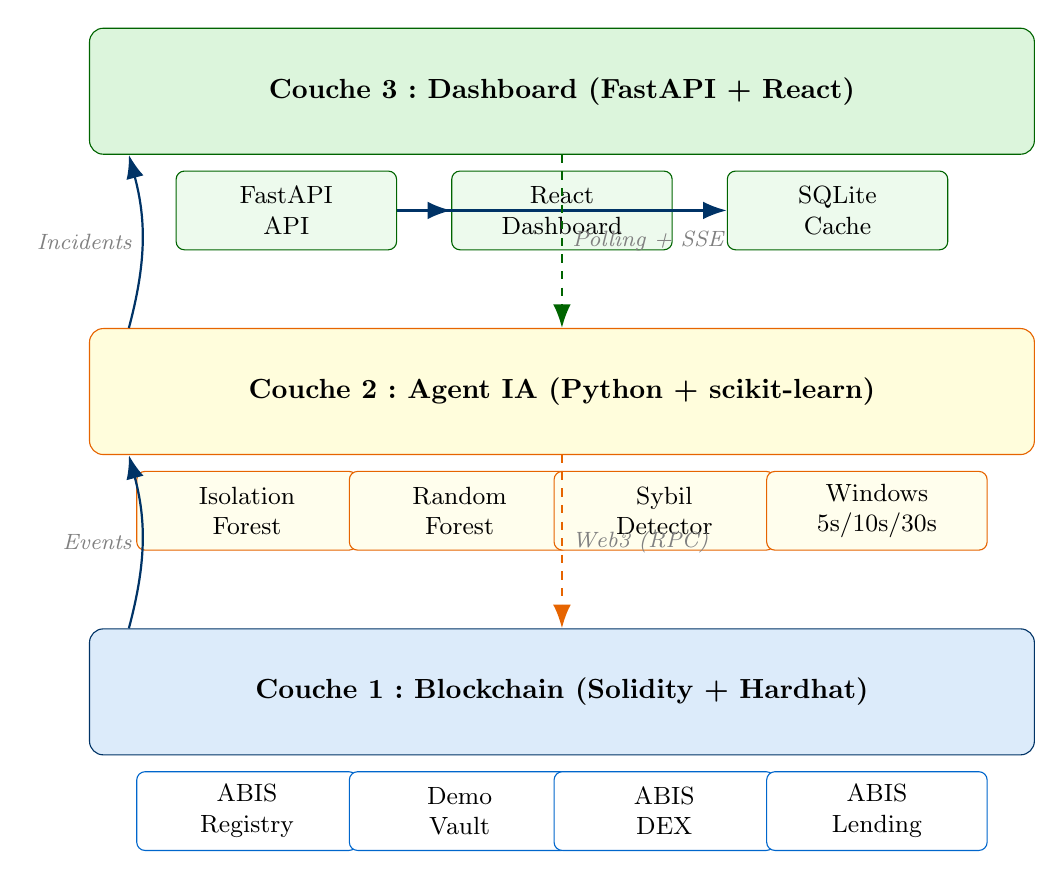
\begin{tikzpicture}[
  node distance=1.5cm,
  layer/.style={rectangle, draw=deepblue, fill=lightblue, rounded corners=5pt,
    minimum width=12cm, minimum height=1.6cm, align=center, font=\bfseries},
  component/.style={rectangle, draw=medblue, fill=white, rounded corners=3pt,
    minimum width=2.8cm, minimum height=1cm, align=center, font=\small},
  arrow/.style={-{Latex[length=3mm]}, thick, color=deepblue},
  label/.style={font=\footnotesize\itshape, color=gray}
]

% Couche 3 - Dashboard
\node[layer, fill=lightgreen, draw=deepgreen] (dash) {Couche 3 : Dashboard (FastAPI + React)};
\node[component, below=0.2cm of dash, xshift=-3.5cm, fill=lightgreen!50, draw=deepgreen] (api) {FastAPI\\API};
\node[component, below=0.2cm of dash, xshift=0cm, fill=lightgreen!50, draw=deepgreen] (ui) {React\\Dashboard};
\node[component, below=0.2cm of dash, xshift=3.5cm, fill=lightgreen!50, draw=deepgreen] (sqlite) {SQLite\\Cache};

% Flèches dashboard
\draw[arrow] (api) -- (ui);
\draw[arrow] (api) -- (sqlite);

% Couche 2 - Agent IA
\node[layer, below=2.2cm of dash, fill=lightyellow, draw=warnorange] (agent) {Couche 2 : Agent IA (Python + scikit-learn)};
\node[component, below=0.2cm of agent, xshift=-4cm, fill=lightyellow!50, draw=warnorange] (if) {Isolation\\Forest};
\node[component, below=0.2cm of agent, xshift=-1.3cm, fill=lightyellow!50, draw=warnorange] (rf) {Random\\Forest};
\node[component, below=0.2cm of agent, xshift=1.3cm, fill=lightyellow!50, draw=warnorange] (sybil) {Sybil\\Detector};
\node[component, below=0.2cm of agent, xshift=4cm, fill=lightyellow!50, draw=warnorange] (windows) {Windows\\5s/10s/30s};

% Couche 1 - Blockchain
\node[layer, below=2.2cm of agent] (chain) {Couche 1 : Blockchain (Solidity + Hardhat)};
\node[component, below=0.2cm of chain, xshift=-4cm] (registry) {ABIS\\Registry};
\node[component, below=0.2cm of chain, xshift=-1.3cm] (vault) {Demo\\Vault};
\node[component, below=0.2cm of chain, xshift=1.3cm] (dex) {ABIS\\DEX};
\node[component, below=0.2cm of chain, xshift=4cm] (lending) {ABIS\\Lending};

% Flèches inter-couches
\draw[arrow, dashed, color=deepgreen] (dash) -- node[right, label]{Polling + SSE} (agent);
\draw[arrow, dashed, color=warnorange] (agent) -- node[right, label]{Web3 (RPC)} (chain);
\draw[arrow, color=deepblue, bend right=15] ([xshift=-5.5cm]chain.north) to node[left, label]{Events} ([xshift=-5.5cm]agent.south);
\draw[arrow, color=deepblue, bend right=15] ([xshift=-5.5cm]agent.north) to node[left, label]{Incidents} ([xshift=-5.5cm]dash.south);

\end{tikzpicture}
\caption{Architecture à trois couches d'ABIS}
\label{fig:architecture_globale}
\end{figure}

\section{Flux de Données}

Le flux de traitement d'une transaction suit un chemin précis à travers les trois couches :

\begin{enumerate}
  \item \textbf{Transaction émise} : Un utilisateur (ou attaquant) envoie une transaction vers un contrat protégé (Vault, DEX, Lending, Token).
  \item \textbf{Exécution du smart contract} : Le modificateur \code{abisGuard} appelle \code{enforceAccess()} sur le registre ABIS, vérifiant le statut du wallet (bloqué, gelé, averti).
  \item \textbf{Événement blockchain} : Si la transaction est autorisée, un événement est émis (ou non émis si bloquée au niveau contrat). L'agent surveille les blocs.
  \item \textbf{Scoring ML} : L'agent extrait les features de la transaction, calcule le risk score via le scoring hybride (IsolationForest + RandomForest).
  \item \textbf{Décision d'enforcement} : Si le risque dépasse le seuil applicable (adapté à la réputation), l'agent appelle la fonction d'enforcement appropriée sur ABISRegistry.
  \item \textbf{Transaction d'enforcement} : ABISRegistry met à jour l'état du wallet (warned/blocked/frozen) et émet un événement \code{IncidentLogged}.
  \item \textbf{Propagation} : Toutes les nouvelles transactions du wallet vers les contrats protégés sont désormais bloquées au niveau EVM.
  \item \textbf{Dashboard} : L'API détecte le nouvel incident via polling des événements blockchain, l'indexe en SQLite, et pousse la mise à jour vers le frontend via SSE.
\end{enumerate}

\begin{figure}[H]
\centering
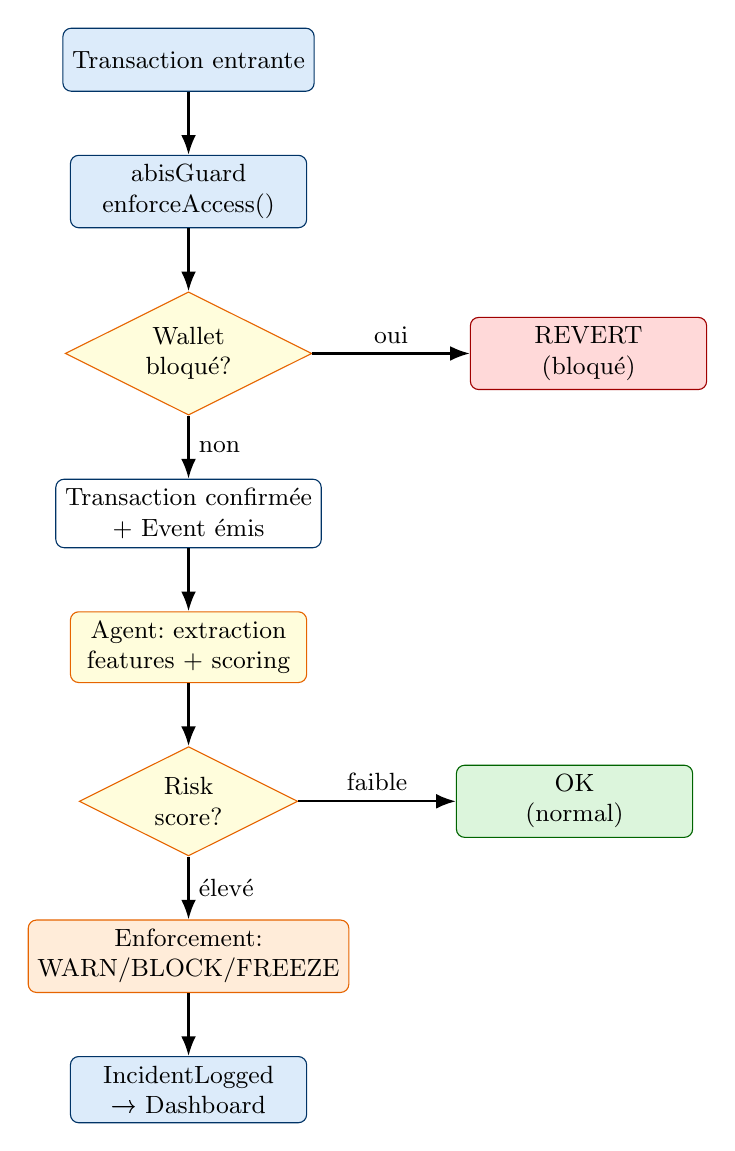
\begin{tikzpicture}[
  node distance=0.8cm,
  box/.style={rectangle, draw=deepblue, rounded corners=3pt,
    minimum width=3cm, minimum height=0.8cm, align=center, font=\small},
  decision/.style={diamond, draw=warnorange, fill=lightyellow,
    minimum width=2.5cm, minimum height=0.8cm, align=center, font=\small, aspect=2},
  arrow/.style={-{Latex[length=2.5mm]}, thick},
]
\node[box, fill=lightblue] (tx) {Transaction entrante};
\node[box, below=of tx, fill=lightblue] (guard) {abisGuard\\ enforceAccess()};
\node[decision, below=of guard] (blocked) {Wallet\\ bloqué?};
\node[box, right=2cm of blocked, fill=red!15, draw=deepred] (revert) {REVERT\\(bloqué)};
\node[box, below=of blocked] (event) {Transaction confirmée\\ + Event émis};
\node[box, below=of event, fill=lightyellow, draw=warnorange] (agent) {Agent: extraction\\ features + scoring};
\node[decision, below=of agent] (risk) {Risk\\ score?};
\node[box, right=2cm of risk, fill=lightgreen, draw=deepgreen] (ok) {OK\\(normal)};
\node[box, below=of risk, fill=orange!15, draw=warnorange] (enforce) {Enforcement:\\ WARN/BLOCK/FREEZE};
\node[box, below=of enforce, fill=lightblue] (incident) {IncidentLogged\\ → Dashboard};

\draw[arrow] (tx) -- (guard);
\draw[arrow] (guard) -- (blocked);
\draw[arrow] (blocked) -- node[right]{\small non} (event);
\draw[arrow] (blocked) -- node[above]{\small oui} (revert);
\draw[arrow] (event) -- (agent);
\draw[arrow] (agent) -- (risk);
\draw[arrow] (risk) -- node[right]{\small élevé} (enforce);
\draw[arrow] (risk) -- node[above]{\small faible} (ok);
\draw[arrow] (enforce) -- (incident);
\end{tikzpicture}
\caption{Flux de traitement d'une transaction par ABIS}
\label{fig:flux_traitement}
\end{figure}

\section{Décisions d'Architecture}

\subsection{Pourquoi Hardhat plutôt qu'un Testnet Public ?}

Le choix d'un nœud Hardhat local (plutôt que Goerli, Sepolia ou un fork mainnet) est justifié par plusieurs raisons :

\begin{itemize}
  \item \textbf{Contrôle total} : Hardhat permet de contrôler le temps de bloc, de miner instantanément, et d'impersonifier n'importe quel compte. Indispensable pour les tests reproductibles.
  \item \textbf{Performance} : Les testnets publics ont des latences réseau variables et des limites de transactions par minute. En local, 70 transactions peuvent être minées en quelques secondes.
  \item \textbf{Isolation} : Pas de dépendance à une infrastructure externe. Le projet est entièrement auto-contenu.
  \item \textbf{Coût} : Pas de frais de gas réels (même sur testnet, les faucets ont des limites).
\end{itemize}

\subsection{Pourquoi Trois Couches Indépendantes ?}

L'architecture en couches découplées offre :
\begin{itemize}
  \item \textbf{Séparation des responsabilités} : Le smart contract gère l'enforcement, l'agent gère la détection, le dashboard gère la présentation. Chacun peut évoluer indépendamment.
  \item \textbf{Résilience} : Si le dashboard tombe, la protection continue (agent + blockchain fonctionnent toujours). Si l'agent redémarre, les états blockchain persistent.
  \item \textbf{Testabilité} : Chaque couche peut être testée séparément.
\end{itemize}

\subsection{Pourquoi un Modificateur \code{abisGuard} ?}

L'alternative aurait été un proxy pattern (comme OpenZeppelin Upgradeable) ou un oracle externe. Le modificateur a été préféré car :
\begin{itemize}
  \item \textbf{Zero-overhead sur lecture} : Les fonctions \code{view/pure} ne nécessitent pas de protection.
  \item \textbf{Atomicité} : La vérification et la transaction sont atomiques. Impossible de contourner par race condition.
  \item \textbf{Lisibilité} : Un seul mot-clé suffit pour protéger une fonction, réduisant le risque d'oubli.
\end{itemize}

\section{Infrastructure et Déploiement}

\subsection{Docker Compose}

L'ensemble du système est orchestré via Docker Compose, définissant 5 services :

\begin{table}[H]
\centering
\caption{Services Docker Compose d'ABIS}
\label{tab:docker_services}
\begin{tabularx}{\linewidth}{L{3cm} L{3cm} L{2cm} L{5cm}}
\toprule
\textbf{Service} & \textbf{Image} & \textbf{Port} & \textbf{Rôle} \\
\midrule
blockchain & node:20-alpine & 8545 & Nœud Hardhat local \\
deploy & node:20-alpine & --- & Déploiement one-shot des contrats \\
agent & python:3.11-slim & --- & Agent ML de surveillance \\
api & python:3.11-slim & 8000 & API REST + SSE \\
frontend & nginx:alpine & 3000 & Interface utilisateur \\
\bottomrule
\end{tabularx}
\end{table}

\subsection{Script de Démarrage}

Le script \code{start.sh} automatise le démarrage en mode développement via tmux :
\begin{enumerate}
  \item Démarre Hardhat et attend la disponibilité du port 8545.
  \item Lance le déploiement des contrats et attend la création de \code{localhost.json}.
  \item Lance l'agent Python et attend le message \code{models\_loaded} dans les logs.
  \item Lance l'API FastAPI.
  \item Lance le frontend Vite.
  \item Ouvre un tmux 4 panes avec chaque service visible.
\end{enumerate}

%% ─────────────────────────────────────────────────────────────────────────────
\chapter{Couche Blockchain : Smart Contracts}
\vspace{0pt}
\vspace{1cm}
%% ─────────────────────────────────────────────────────────────────────────────

\section{Vue d'Ensemble des Contrats}

La couche blockchain d'ABIS comprend cinq smart contracts développés en Solidity 0.8.24, déployés sur un nœud Hardhat local. Ces contrats forment deux catégories distinctes :

\begin{itemize}
  \item \textbf{Contrat central} : \code{ABISRegistry} -- gère toute la logique de sécurité (statuts, réputation, incidents).
  \item \textbf{Contrats DeFi de démonstration} : \code{DemoVault}, \code{ABISDex}, \code{ABISLending}, \code{ABISToken} -- simulent des protocoles réels protégés par ABIS.
\end{itemize}

\begin{table}[H]
\centering
\caption{Smart Contracts ABIS}
\label{tab:contracts}
\begin{tabularx}{\linewidth}{L{3.5cm} C{1.5cm} L{7.5cm}}
\toprule
\textbf{Contrat} & \textbf{Lignes} & \textbf{Rôle} \\
\midrule
ABISRegistry & 294 & Registre central : statuts wallets, incidents, whitelist, circuit breaker \\
DemoVault & 52 & Coffre de dépôt/retrait ETH avec abisGuard \\
ABISDex & 68 & Exchange décentralisé simplifié (AMM) \\
ABISLending & 86 & Protocole de prêt/emprunt avec collatéral \\
ABISToken & 45 & Token ERC-20 standard protégé \\
\bottomrule
\end{tabularx}
\end{table}

\section{ABISRegistry : Le Contrat Central}

\subsection{Structures de Données}

\code{ABISRegistry} maintient l'état de sécurité de l'ensemble du système à travers plusieurs mappings :

\begin{lstlisting}[language=Solidity, caption={Structures principales d'ABISRegistry}, label={lst:registry_structs}]
// Statut par wallet
struct WalletStatus {
    bool isBlocked;
    bool isFrozen;
    bool isWarned;
    uint256 blockExpiry;
    uint256 warnExpiry;
    uint256 txDelaySeconds;
    uint256 lastTxTimestamp;
    uint256 riskScore;
    string lastReason;
    bytes32 lastProtocol;
}

mapping(address => WalletStatus) public walletStatus;

// Blocages par protocole
mapping(address => mapping(bytes32 => uint256)) public protocolBlockExpiry;

// Réputation
mapping(address => uint256) public walletReputation;

// Incidents
mapping(uint256 => IncidentRecord) public incidents;
uint256 public incidentCount;

// Whitelist
mapping(address => bool) public whitelist;

// Circuit breaker
bool public isPaused;
\end{lstlisting}

\subsection{Système d'Enforcement à Quatre Niveaux}

ABIS définit quatre niveaux de réponse proportionnels à la sévérité du risque détecté :

\begin{table}[H]
\centering
\caption{Niveaux d'enforcement ABIS}
\label{tab:enforcement_levels}
\begin{tabularx}{\linewidth}{C{1.5cm} C{2.5cm} C{2cm} L{6.5cm}}
\toprule
\textbf{Niveau} & \textbf{Action} & \textbf{Seuil} & \textbf{Effet} \\
\midrule
L0 & Normal   & < 40  & Aucune action \\
L1 & WARN     & 40--64 & Rate-limit : 2 min de fenêtre, 30s de délai entre tx \\
L2 & BLOCK    & 65--91 & Blocage global de 10 minutes sur tous les protocoles \\
L2b & BLOCK\_PROTOCOL & 65--91 & Blocage de 10 minutes sur un protocole spécifique \\
L3 & FREEZE   & $\geq$ 92 & Gel permanent jusqu'à intervention manuelle \\
\bottomrule
\end{tabularx}
\end{table}

\begin{lstlisting}[language=Solidity, caption={Fonction warnWallet}, label={lst:warn_wallet}]
function warnWallet(
    address wallet,
    uint256 windowSeconds,
    uint256 txDelaySeconds,
    uint256 riskScore,
    string calldata reason
) external onlyOwner notPaused notWhitelisted(wallet) {
    WalletStatus storage s = walletStatus[wallet];
    s.isWarned = true;
    s.warnExpiry = block.timestamp + windowSeconds;
    s.txDelaySeconds = txDelaySeconds;
    s.riskScore = riskScore;
    s.lastReason = reason;
    _logIncident(wallet, "WARN", riskScore, reason);
    emit WalletWarned(wallet, block.timestamp + windowSeconds, riskScore, reason);
}
\end{lstlisting}

\begin{lstlisting}[language=Solidity, caption={Fonction blockWallet}, label={lst:block_wallet}]
function blockWallet(
    address wallet,
    uint256 durationSeconds,
    uint256 riskScore,
    string calldata reason
) external onlyOwner notPaused notWhitelisted(wallet) {
    WalletStatus storage s = walletStatus[wallet];
    s.isBlocked = true;
    s.blockExpiry = block.timestamp + durationSeconds;
    s.riskScore = riskScore;
    s.lastReason = reason;
    walletReputation[wallet]++;
    _logIncident(wallet, "BLOCK", riskScore, reason);
    emit WalletBlocked(wallet, block.timestamp + durationSeconds, riskScore, reason);
}
\end{lstlisting}

\begin{lstlisting}[language=Solidity, caption={Fonction freezeWallet}, label={lst:freeze_wallet}]
function freezeWallet(
    address wallet,
    uint256 riskScore,
    string calldata reason
) external onlyOwner notPaused notWhitelisted(wallet) {
    WalletStatus storage s = walletStatus[wallet];
    s.isFrozen = true;
    s.riskScore = riskScore;
    s.lastReason = reason;
    walletReputation[wallet]++;
    _logIncident(wallet, "FREEZE", riskScore, reason);
    emit WalletFrozen(wallet, riskScore, reason);
}
\end{lstlisting}

\subsection{Modificateur abisGuard}

Le cœur de la protection au niveau smart contract est le modificateur \code{abisGuard}, appliqué à chaque fonction sensible des contrats DeFi :

\begin{lstlisting}[language=Solidity, caption={Modificateur abisGuard et enforceAccess}, label={lst:abis_guard}]
modifier abisGuard(bytes32 protocol) {
    registry.enforceAccess(msg.sender, protocol);
    _;
}

// Dans ABISRegistry :
function enforceAccess(address wallet, bytes32 protocol)
    external view
{
    if (isPaused) return; // Circuit breaker actif
    if (whitelist[wallet]) return; // Wallet whitelisté

    WalletStatus storage s = walletStatus[wallet];

    // Vérification gel permanent
    require(!s.isFrozen, "ABIS: wallet permanently frozen");

    // Vérification blocage global (avec expiry)
    if (s.isBlocked && block.timestamp < s.blockExpiry) {
        revert("ABIS: wallet globally blocked");
    }

    // Vérification blocage par protocole
    if (protocolBlockExpiry[wallet][protocol] > block.timestamp) {
        revert("ABIS: wallet blocked on this protocol");
    }

    // Vérification rate-limit (avertissement)
    if (s.isWarned && block.timestamp < s.warnExpiry) {
        require(
            block.timestamp >= s.lastTxTimestamp + s.txDelaySeconds,
            "ABIS: rate-limit active, wait before next tx"
        );
    }

    // Mise a jour du timestamp
    walletStatus[wallet].lastTxTimestamp = block.timestamp;
}
\end{lstlisting}

\subsection{Profil de Wallet et Requête Complète}

\code{ABISRegistry} expose une fonction \code{getWalletProfile()} qui retourne un tuple de 10 valeurs, permettant au dashboard d'afficher l'état complet d'un wallet en un seul appel. Cette fonction nécessite la directive \code{viaIR: true} dans \code{hardhat.config.js} pour éviter l'erreur \textit{Stack too deep} du compilateur Solidity lors de la construction d'un return tuple aussi large.

\subsection{Événements et Logging On-Chain}

Tous les événements de sécurité sont enregistrés on-chain via l'événement \code{IncidentLogged} :

\begin{lstlisting}[language=Solidity, caption={Événement IncidentLogged}, label={lst:incident_logged}]
event IncidentLogged(
    uint256 indexed incidentId,
    address indexed wallet,
    string action,
    uint256 riskScore,
    string reason,
    uint256 timestamp
);

struct IncidentRecord {
    address wallet;
    string action;
    uint256 riskScore;
    string reason;
    uint256 timestamp;
}
\end{lstlisting}

Le champ \code{reason} contient une chaîne de caractères structurée de type clé=valeur, parsée par l'API pour extraire les métriques de détection :

\begin{codebox}[Exemple de reason string]
\small\texttt{protocol=Vault attack\_type=burst\_dex\_same method=classifier risk=84.2 window=30s cnt30s=12 unique\_to=1 same\_to=11 confidence=0.923 repeat\_offender=2 sybil\_wallets=3 long\_window\_boost=15.0}
\end{codebox}

\section{Contrats DeFi de Démonstration}

\subsection{DemoVault}

\code{DemoVault} simule un coffre de rendement simple permettant dépôts et retraits d'ETH. Chaque opération est protégée par \code{abisGuard("VAULT")} :

\begin{lstlisting}[language=Solidity, caption={DemoVault.sol (simplifié)}, label={lst:demo_vault}]
contract DemoVault {
    ABISRegistry public registry;
    mapping(address => uint256) public balances;

    function deposit() external payable abisGuard("VAULT") {
        require(msg.value > 0, "DemoVault: zero deposit");
        balances[msg.sender] += msg.value;
        emit Deposited(msg.sender, msg.value);
    }

    function withdraw(uint256 amount) external abisGuard("VAULT") {
        require(balances[msg.sender] >= amount, "Insufficient balance");
        balances[msg.sender] -= amount;
        payable(msg.sender).transfer(amount);
        emit Withdrawn(msg.sender, amount);
    }
}
\end{lstlisting}

\subsection{ABISDex}

\code{ABISDex} implémente un AMM simplifié avec un pool ETH/ABST. Il expose les fonctions \code{buyTokens()} et \code{sellTokens()}, chacune protégée par \code{abisGuard("DEX")}. Le prix est calculé selon la formule $x \times y = k$ : \texttt{tokensOut = tokenReserve * ethIn / (ethReserve + ethIn)}.

\subsection{ABISLending}

\code{ABISLending} simule un protocole de prêt/emprunt avec collatéral. Il maintient les dépôts de collatéral, les positions d'emprunt, et calcule le LTV (\textit{Loan-to-Value}) pour chaque wallet. Les fonctions de dépôt, retrait et emprunt sont toutes protégées par \code{abisGuard("LENDING")}.

\section{Considérations de Sécurité}

\subsection{Protections Contre les Attaques Communes}

\begin{itemize}
  \item \textbf{Reentrancy} : Le pattern \textit{Checks-Effects-Interactions} est appliqué dans toutes les fonctions de retrait. Les modifications d'état précèdent les transferts ETH.
  \item \textbf{Integer Overflow} : Solidity 0.8.x intègre des vérifications overflow nativement (revert automatique).
  \item \textbf{Access Control} : Le modificateur \code{onlyOwner} (Ownable d'OpenZeppelin) protège toutes les fonctions d'administration d'ABISRegistry.
  \item \textbf{Pull over Push} : Les retraits utilisent le pattern pull (\code{withdraw()}) plutôt que push pour éviter les blocages de fonds.
\end{itemize}

\subsection{Circuit Breaker}

Le circuit breaker (\code{isPaused}) permet à l'administrateur de suspendre immédiatement toutes les protections ABIS, par exemple pour maintenance ou en cas de bug dans l'agent. Contrairement au circuit breaker des protocoles DeFi classiques (qui stoppe les opérations), celui d'ABIS ne bloque pas le protocole --- il désactive temporairement les vérifications de sécurité, ce qui est l'opposé du sens usuel mais cohérent avec le rôle d'ABIS comme surcouche de sécurité.

%% ─────────────────────────────────────────────────────────────────────────────
\chapter{Couche Intelligence Artificielle}
\vspace{0pt}
\vspace{1cm}
%% ─────────────────────────────────────────────────────────────────────────────

\section{Architecture de l'Agent}

L'agent ABIS (\code{abis\_agent.py}, 668 lignes) est un processus Python autonome qui :
\begin{enumerate}
  \item Se connecte au nœud Ethereum via Web3.py (JSON-RPC sur port 8545).
  \item Charge six objets ML sérialisés (fichiers \code{.pkl}).
  \item Entre dans une boucle infinie de surveillance bloc-par-bloc.
  \item Pour chaque transaction dans chaque nouveau bloc, extrait les features, calcule un score de risque, et décide d'une action d'enforcement.
\end{enumerate}

\begin{infobox}[Séquence de démarrage de l'agent]
\begin{enumerate}
  \item Chargement de \code{wallet\_reputation.json} (historique des récidivistes)
  \item Chargement des 6 modèles ML (IsolationForest, scalers, RandomForest, labels)
  \item Log : \texttt{\{"event": "models\_loaded", "attack\_types": 48\}}
  \item Boucle \code{connect()} → bloque jusqu'à la disponibilité de Hardhat
  \item Détermination du compte admin : variable d'env \code{AGENT\_PRIVATE\_KEY} ou \code{w3.eth.accounts[0]}
  \item Entrée dans la boucle principale de scan des blocs
\end{enumerate}
\end{infobox}

\section{Pipeline de Données ML}

\subsection{Génération du Dataset Normal}

Le dataset d'entraînement pour l'IsolationForest est généré par \code{generate\_normal\_dataset.py}, produisant 170\,000 lignes représentant 8 archétypes d'utilisateurs normaux :

\begin{table}[H]
\centering
\caption{Archétypes d'utilisateurs normaux}
\label{tab:normal_archetypes}
\begin{tabularx}{\linewidth}{L{4cm} C{2cm} L{7cm}}
\toprule
\textbf{Archétype} & \textbf{Samples} & \textbf{Comportement typique} \\
\midrule
casual\_user & 25\,000 & Dépôts occasionnels, petits montants \\
defi\_trader & 25\,000 & Transactions fréquentes, montants variables \\
liquidity\_provider & 20\,000 & Dépôts/retraits réguliers, montants moyens \\
hodler & 15\,000 & Transactions très espacées, gros montants \\
token\_user & 25\,000 & Transferts de tokens, cibles diverses \\
lender\_borrower & 20\,000 & Dépôts collatéral, emprunts réguliers \\
multi\_protocol & 25\,000 & Utilise tous les protocoles alternativement \\
power\_user & 15\,000 & Volume élevé, diversité des actions \\
\midrule
\textbf{Total} & \textbf{170\,000} & \\
\bottomrule
\end{tabularx}
\end{table}

\subsection{Génération du Dataset d'Attaques}

\code{generate\_attack\_dataset.py} génère 150\,000 échantillons d'attaques : 48 types $\times$ 3\,125 samples par type. Les features sont synthétisées en simulant les statistiques de fenêtres glissantes caractéristiques de chaque type d'attaque.

\section{Extraction de Features}

\subsection{Les 9 Features d'ABIS}

Pour chaque transaction, l'agent maintient des historiques glissants par wallet pour trois fenêtres temporelles [5s, 10s, 30s]. Pour chaque fenêtre $W$, 9 features sont extraites :

\begin{table}[H]
\centering
\caption{Features extraites par l'agent ABIS}
\label{tab:features}
\begin{tabularx}{\linewidth}{L{4cm} C{2cm} L{7cm}}
\toprule
\textbf{Feature} & \textbf{Type} & \textbf{Description} \\
\midrule
\code{tx\_count\_w} & int & Nombre de tx dans la fenêtre W \\
\code{avg\_value\_w} & float & Montant moyen en ETH sur W \\
\code{std\_value\_w} & float & Écart-type des montants sur W \\
\code{dt\_prev} & float & Délai depuis la tx précédente (s) ; 999999 si première \\
\code{value\_eth} & float & Montant de la tx courante en ETH \\
\code{unique\_to\_w} & int & Nombre de destinataires distincts sur W \\
\code{same\_to\_burst\_w} & int & Nb de tx vers le même destinataire sur W \\
\code{contract\_target} & int & Encodage du contrat cible (0=Vault, 1=DEX, 2=Lending, 3=Token) \\
\code{window\_s} & float & Durée de la fenêtre en secondes (5.0, 10.0, ou 30.0) \\
\bottomrule
\end{tabularx}
\end{table}

\subsection{Justification du Choix des Features}

\begin{itemize}
  \item \code{tx\_count\_w} et \code{dt\_prev} : Capturent la fréquence des transactions, discriminant les attaques de type burst.
  \item \code{std\_value\_w} : Les attaques ont souvent des montants très variables (pump\&dump) ou très uniformes (griefing). La variance est donc très discriminante.
  \item \code{unique\_to\_w} vs \code{same\_to\_burst\_w} : Distingue le spray (beaucoup de destinataires différents) du burst ciblé (même destinataire à répétition).
  \item \code{value\_eth} seul : Les attaques de type integer overflow probing utilisent des montants extrêmes (1000 ETH).
  \item \code{contract\_target} : Certaines attaques sont spécifiques à un protocole. Permet au modèle d'apprendre les patterns par contexte.
  \item \code{window\_s} : Permet à un même modèle de distinguer des patterns à différentes échelles temporelles.
\end{itemize}

\section{Modèles ML}

\subsection{IsolationForest : Détection Non Supervisée}

L'IsolationForest est entraîné sur les 170\,000 transactions normales \textit{uniquement}, sans aucune donnée d'attaque. Ce choix est fondamental : le modèle apprend ce qu'est la normalité, et toute déviation est une anomalie, qu'elle soit d'un type connu ou inédit.

\begin{itemize}
  \item \textbf{Hyperparamètres} : 400 estimateurs, contamination=0.02, \code{random\_state=42}.
  \item \textbf{Calibration} : Les scores bruts de l'IF (continus, négatifs pour les anomalies) sont convertis en risk scores 0--100 via une calibration sur les percentiles p3 (score minimal observé → risque 100) et p92 (score à 92\% → risque 0). Cette calibration garantit que le seuil de 65 correspond à un niveau d'anomalie statistiquement significatif.
  \item \textbf{Avantage clé} : Détecte des \textit{zero-day attacks} -- des types d'attaque non présents dans le dataset supervisé.
\end{itemize}

\begin{lstlisting}[language=Python, caption={Calibration de l'IsolationForest}, label={lst:if_calibration}]
scores = iforest.score_samples(X_normal_scaled)
p3 = np.percentile(scores, 3)    # score tres anormal -> risque 100
p92 = np.percentile(scores, 92)  # score plutot normal -> risque 0

cal = {"p99": p3, "p1": p92}  # naming interne conserve pour compat.

def score_to_risk(if_score, cal):
    p99, p1 = cal["p99"], cal["p1"]
    risk = 100.0 * np.clip((p99 - if_score) / (p99 - p1), 0.0, 1.0)
    return risk
\end{lstlisting}

\subsection{RandomForest : Classification Supervisée}

Le RandomForest est entraîné sur 150\,000 échantillons labellisés couvrant 48 types d'attaques. Il fournit une probabilité de classification pour chacun des 48 types, permettant d'identifier \textit{quel type} d'attaque est en cours.

\begin{itemize}
  \item \textbf{Hyperparamètres} : 400 estimateurs, \code{class\_weight="balanced"}, \code{min\_samples\_leaf=2}, \code{random\_state=42}.
  \item \textbf{class\_weight="balanced"} : Essentiel car certains types d'attaque (ex. mega\_burst) génèrent beaucoup plus de patterns distincts que d'autres (ex. low\_and\_slow). L'équilibrage empêche le modèle d'être biaisé vers les classes surreprésentées.
  \item \textbf{Avantage clé} : Fournit le label d'attaque affiché dans le dashboard et stocké dans les événements on-chain.
\end{itemize}

\subsection{Scoring Hybride}

L'originalité majeure d'ABIS réside dans son algorithme de scoring hybride, qui combine les deux modèles selon un arbre de décision basé sur la confiance du RF :

\begin{lstlisting}[language=Python, caption={Fonction hybrid\_score}, label={lst:hybrid_score}]
def hybrid_score(row_df):
    # Branche RandomForest
    Xc = clf_scl.transform(row_df.values)
    proba = clf.predict_proba(Xc)[0]
    best_idx = int(np.argmax(proba))
    best_conf = float(proba[best_idx])
    attack_pred = clf_lbl[best_idx]

    # Branche IsolationForest
    Xs = if_scl.transform(row_df.values)
    if_score = float(iforest.score_samples(Xs)[0])
    if_risk = float(score_to_risk(if_score, cal))

    # Arbre de decision
    if best_conf >= 0.75:   # Confiance haute : le RF drive
        risk = 65.0 + (best_conf - 0.75) / 0.25 * 34.0
        risk = min(max(risk, if_risk), 99.0)
        return risk, attack_pred, "classifier", best_conf

    if best_conf >= 0.40:   # Confiance moyenne : IF pour le score, RF pour le label
        return if_risk, attack_pred, "iforest+clf", best_conf

    if if_risk >= 65:       # RF incertain mais IF detecte une anomalie
        return if_risk, "unknown_anomaly", "iforest", None

    return if_risk, "normal", "iforest", None  # Tout est normal
\end{lstlisting}

\begin{figure}[H]
\centering
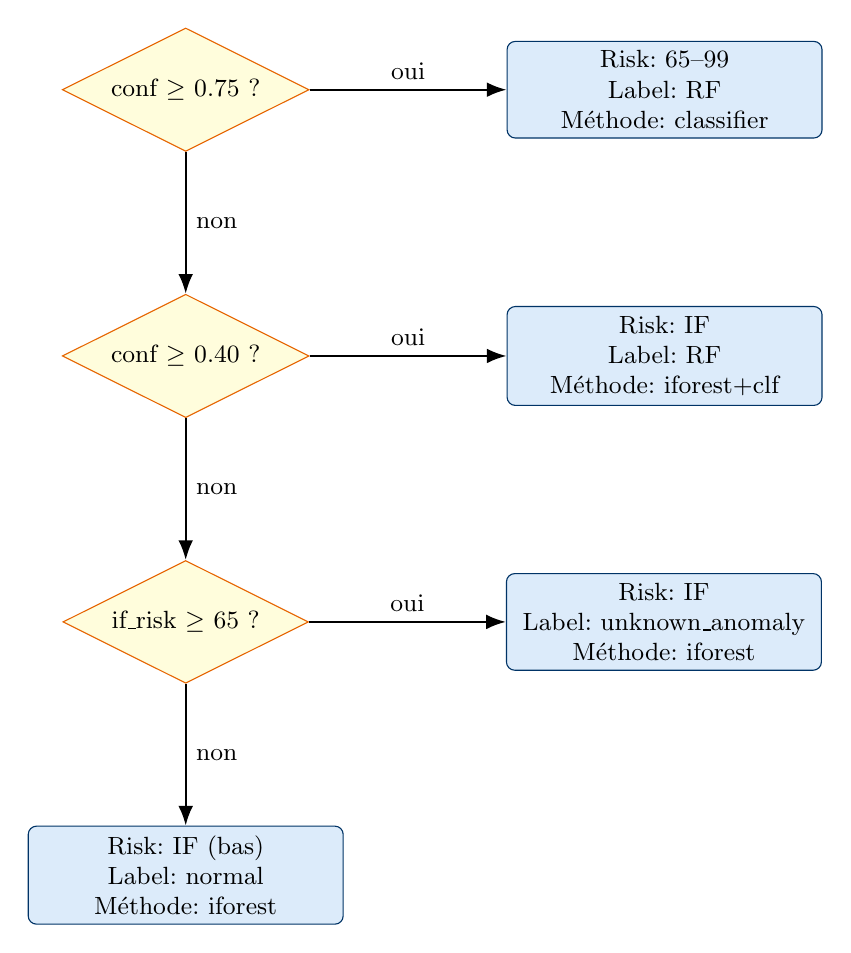
\begin{tikzpicture}[
  node distance=1.2cm,
  decision/.style={diamond, draw=warnorange, fill=lightyellow,
    minimum width=3cm, align=center, font=\small, aspect=2},
  result/.style={rectangle, draw=deepblue, fill=lightblue, rounded corners=3pt,
    minimum width=4cm, minimum height=0.8cm, align=center, font=\small},
  arrow/.style={-{Latex[length=2.5mm]}, thick},
]
\node[decision] (conf1) {conf $\geq$ 0.75 ?};
\node[result, right=2.5cm of conf1] (r1) {Risk: 65--99\\Label: RF\\Méthode: classifier};
\node[decision, below=1.8cm of conf1] (conf2) {conf $\geq$ 0.40 ?};
\node[result, right=2.5cm of conf2] (r2) {Risk: IF\\Label: RF\\Méthode: iforest+clf};
\node[decision, below=1.8cm of conf2] (ifrisk) {if\_risk $\geq$ 65 ?};
\node[result, right=2.5cm of ifrisk] (r3) {Risk: IF\\Label: unknown\_anomaly\\Méthode: iforest};
\node[result, below=1.8cm of ifrisk] (r4) {Risk: IF (bas)\\Label: normal\\Méthode: iforest};

\draw[arrow] (conf1) -- node[above]{\small oui} (r1);
\draw[arrow] (conf1) -- node[right]{\small non} (conf2);
\draw[arrow] (conf2) -- node[above]{\small oui} (r2);
\draw[arrow] (conf2) -- node[right]{\small non} (ifrisk);
\draw[arrow] (ifrisk) -- node[above]{\small oui} (r3);
\draw[arrow] (ifrisk) -- node[right]{\small non} (r4);
\end{tikzpicture}
\caption{Arbre de décision du scoring hybride ABIS}
\label{fig:hybrid_scoring}
\end{figure}

\section{Mécanismes d'Amplification}

\subsection{A1 : Détection Sybil (Coordination Inter-Wallets)}

Le module Sybil d'ABIS détecte la coordination entre plusieurs wallets attaquant simultanément le même protocole avec le même type d'attaque. L'algorithme utilise des buckets temporels de 30 secondes :

\begin{lstlisting}[language=Python, caption={Détection Sybil}, label={lst:sybil_detection}]
def check_sybil_coordination(sender, protocol, attack_type, bt):
    bucket_key = (protocol, attack_type, bt // 30)
    sybil_buckets[bucket_key].add(sender)

    wallet_count = len(sybil_buckets[bucket_key])
    if wallet_count >= 3:
        boost = min(20, wallet_count * 5)
        return True, boost

    # Purge des anciens buckets
    current_slot = bt // 30
    old_keys = [k for k in sybil_buckets if current_slot - k[2] > 5]
    for k in old_keys:
        del sybil_buckets[k]

    return False, 0
\end{lstlisting}

\begin{itemize}
  \item \textbf{Seuil} : 3 wallets ou plus dans le même bucket = coordination confirmée.
  \item \textbf{Boost} : $\min(20, N \times 5)$ où $N$ est le nombre de wallets coordonnés.
  \item \textbf{Justification du bucket de 30s} : C'est la fenêtre maximale des fenêtres courtes d'ABIS. Deux wallets attaquant avec 35s d'écart ne sont pas coordonnés ; à 25s, ils le sont probablement.
\end{itemize}

\subsection{A2 : Détection Low-and-Slow (Longues Fenêtres)}

Les fenêtres courtes (5s, 10s, 30s) ne peuvent pas détecter des attaques qui s'étalent sur plusieurs minutes. ABIS intègre donc deux fenêtres longues [300s, 3600s] avec une logique de boost spécifique :

\begin{lstlisting}[language=Python, caption={Boost long-window}, label={lst:long_window}]
def score_long_window(sender, bt, long_windows):
    max_boost = 0
    for W in long_windows:
        entries = hist_long[sender][W]
        # Filtre des entrees dans la fenetre
        entries = [e for e in entries if bt - e[0] <= W]
        cnt = len(entries)
        if cnt == 0:
            continue
        avg = np.mean([e[1] for e in entries])

        # Pattern low-and-slow : beaucoup de microtx
        if cnt >= 10 and avg < 0.01:
            boost = min(25, cnt * 1.5)
            max_boost = max(max_boost, boost)

        # Pattern gradual escalation : montants croissants
        elif cnt >= 6:
            half = cnt // 2
            first_half = [e[1] for e in entries[:half]]
            second_half = [e[1] for e in entries[half:]]
            if np.mean(second_half) > np.mean(first_half) * 2:
                boost = 15.0
                max_boost = max(max_boost, boost)

    return max_boost
\end{lstlisting}

\section{Système de Réputation}

\subsection{Principe}

La réputation d'un wallet affecte son seuil de blocage. Un récidiviste est sanctionné plus tôt :

\begin{table}[H]
\centering
\caption{Impact de la réputation sur le seuil de blocage}
\label{tab:reputation}
\begin{tabular}{ccc}
\toprule
\textbf{Blocages antérieurs} & \textbf{Seuil appliqué} & \textbf{Facteur} \\
\midrule
0 & 65 & $\times 1.00$ \\
1 & 48.75 & $\times 0.75$ \\
$\geq 2$ & 35.75 & $\times 0.55$ \\
\bottomrule
\end{tabular}
\end{table}

La réputation est persistée dans \code{wallet\_reputation.json} et survivant aux redémarrages de l'agent. Elle est chargée au démarrage et mise à jour après chaque BLOCK ou FREEZE.

\subsection{Cooldown}

Pour éviter de spammer la blockchain avec des transactions d'enforcement, un cooldown de 60 secondes est appliqué par wallet. L'escalade de niveau (WARN → BLOCK → FREEZE) contourne ce cooldown.

\section{Apprentissage en Ligne (Online Learning)}

\subsection{Pipeline de Réentraînement}

ABIS intègre un mécanisme d'apprentissage en ligne pour s'adapter aux nouvelles attaques détectées :

\begin{enumerate}
  \item Chaque attaque détectée (avec ses features et son label) est bufferisée dans \code{new\_attacks\_buffer.csv}.
  \item Quand 50 nouvelles samples sont accumulées, un réentraînement est déclenché en arrière-plan (thread séparé).
  \item Le script \code{train\_classifier\_fast.py} est exécuté : il fusionne le buffer avec le dataset principal, réentraîne un RF à 200 arbres (plus rapide), et sauvegarde les nouveaux modèles.
  \item À la fin, \code{models.reload\_classifier()} effectue un hot-swap atomique (via \code{threading.Lock}) des modèles en mémoire.
\end{enumerate}

\begin{warningbox}[Limitation connue]
Le réentraînement online utilise des chemins relatifs (\code{Path("../data/...")}), ce qui le rend dépendant du répertoire de travail. En production, ces chemins devraient être configurés via des variables d'environnement.
\end{warningbox}

\section{Les 48 Types d'Attaques}

ABIS couvre 48 types d'attaques répartis en 10 catégories. Le tableau suivant présente une sélection représentative :

\begin{table}[H]
\centering
\caption{Catégories d'attaques couvertes par ABIS (sélection)}
\label{tab:attack_categories}
\begin{tabularx}{\linewidth}{L{2.5cm} C{1.5cm} L{9cm}}
\toprule
\textbf{Catégorie} & \textbf{Nombre} & \textbf{Types inclus} \\
\midrule
Burst & 7 & burst\_dex\_same, burst\_token\_same, burst\_vault\_same, burst\_lending\_same, burst\_wallet\_same, micro\_burst, mega\_burst \\
Spray & 5 & spray\_token\_multi, spray\_eth\_multi, spray\_vault\_multi, spray\_dex\_multi, fan\_out\_attack \\
Prix & 5 & pump\_dump\_token, wash\_trading, price\_slippage\_abuse, sandwich\_attack, front\_running \\
Liquidité & 3 & liquidity\_drain, liquidity\_inject\_withdraw, pool\_imbalance\_attack \\
Lending & 5 & borrow\_max\_ltv, collateral\_dump, flash\_borrow\_repay, liquidation\_trigger, debt\_loop \\
Sybil & 4 & sybil\_attack, new\_wallet\_burst, coordinated\_wallets, relay\_attack \\
Drainage & 5 & vault\_drain, token\_drain, wallet\_drain\_slow, wallet\_drain\_fast, contract\_drain \\
Furtif & 5 & low\_and\_slow, gradual\_escalation, periodic\_bot, night\_owl, stealth\_accumulation \\
Exploits & 5 & reentrancy\_simulation, integer\_overflow\_probe, zero\_value\_spam, gas\_griefing, contract\_call\_flood \\
MEV & 4 & mev\_bot\_pattern, arbitrage\_aggressive, sniper\_bot, block\_stuffing \\
\bottomrule
\end{tabularx}
\end{table}

%% ─────────────────────────────────────────────────────────────────────────────
\chapter{Couche Dashboard : API et Interface}
\vspace{0pt}
\vspace{1cm}
%% ─────────────────────────────────────────────────────────────────────────────

\section{API FastAPI}

\subsection{Architecture de l'API}

L'API ABIS (\code{main.py}, 1105 lignes) est développée avec FastAPI et expose 25+ endpoints REST ainsi qu'un endpoint Server-Sent Events (SSE). Elle joue le rôle d'intermédiaire entre la blockchain et le frontend :

\begin{enumerate}
  \item \textbf{Lecture blockchain} : Query des événements \code{IncidentLogged} via Web3.py.
  \item \textbf{Cache SQLite} : Indexation des événements dans \code{abis\_cache.db} pour des requêtes rapides.
  \item \textbf{Cache RAM} : TTL de 2 secondes pour éviter de requêter SQLite à chaque polling.
  \item \textbf{Exposition REST + SSE} : Sert le dashboard React.
\end{enumerate}

\subsection{Endpoints Principaux}

\begin{table}[H]
\centering
\caption{Principaux endpoints de l'API ABIS}
\label{tab:api_endpoints}
\begin{tabularx}{\linewidth}{L{5cm} C{1.5cm} L{6.5cm}}
\toprule
\textbf{Endpoint} & \textbf{Méthode} & \textbf{Description} \\
\midrule
\code{/health} & GET & État du système (blockchain, cache, version) \\
\code{/metrics} & GET & Compteurs globaux (incidents, bloqués, gelés) \\
\code{/incidents} & GET & Liste des incidents (paginée, filtrée) \\
\code{/blocked-wallets} & GET & Wallets actuellement bloqués \\
\code{/frozen-wallets} & GET & Wallets gelés (permanent) \\
\code{/warned-wallets} & GET & Wallets sous rate-limit \\
\code{/protocol-blocks} & GET & Blocages par protocole \\
\code{/timeline} & GET & Historique des risk scores par bloc \\
\code{/stats} & GET & Statistiques avancées (distributions) \\
\code{/wallet/\{addr\}} & GET & Profil complet d'un wallet \\
\code{/whitelist} & GET/POST/DELETE & Gestion de la whitelist \\
\code{/circuit-breaker} & GET/POST & État et toggle du circuit breaker \\
\code{/unblock/\{addr\}} & POST & Déblocage manuel d'un wallet \\
\code{/unfreeze/\{addr\}} & POST & Dégel manuel d'un wallet \\
\code{/attack/list} & GET & Liste des 48 types d'attaques \\
\code{/attack/run} & POST & Lancer une attaque simulée (SSE stream) \\
\code{/events/stream} & GET & SSE : push métriques + nouveaux incidents \\
\bottomrule
\end{tabularx}
\end{table}

\subsection{Sécurité de l'API}

\begin{itemize}
  \item \textbf{Rate Limiting} : 120 requêtes/minute global, 60/minute sur \code{/incidents}.
  \item \textbf{CORS} : Origines autorisées uniquement \code{:5173} et \code{:4173} (Vite dev + preview).
  \item \textbf{Validation des adresses} : Regex \texttt{\^0x[a-fA-F0-9]\{40\}\$} sur toutes les adresses.
  \item \textbf{Protection path traversal} : \code{/attack/run} valide le nom de l'attaque contre une whitelist (\code{attacks\_meta.json}) et rejette tout chemin contenant \texttt{..} ou \texttt{/}.
\end{itemize}

\begin{warningbox}[Vulnérabilité connue]
Les endpoints \code{/unblock} et \code{/unfreeze} ne requièrent pas d'authentification. Dans un déploiement de production, une signature admin ou une clé API serait nécessaire.
\end{warningbox}

\subsection{Server-Sent Events (SSE)}

L'endpoint \code{/events/stream} implémente une connexion SSE persistante qui pousse deux types d'événements vers le frontend :

\begin{itemize}
  \item \textbf{\code{metrics}} : Mise à jour des compteurs globaux, émise toutes les 2 secondes.
  \item \textbf{\code{new\_incidents}} : Notification de nouveaux incidents, déclenche un rechargement côté client.
\end{itemize}

Ce mécanisme permet au dashboard de rester synchronisé avec la blockchain sans polling intensif. En cas de déconnexion SSE, le frontend bascule automatiquement en mode polling.

\section{Interface React}

\subsection{Architecture Technique}

Le frontend est une Single Page Application (SPA) développée avec React 19 et Vite 7 :
\begin{itemize}
  \item \textbf{Gestion d'état} : 100\% \code{useState/useEffect} -- pas de Redux ou Zustand. Justification : la complexité de l'application ne justifie pas l'overhead d'une bibliothèque de state management.
  \item \textbf{Navigation} : Variable \code{activeTab} (pas de React Router). Justification : application monolithique à 4 onglets, pas de besoins d'URL profonde.
  \item \textbf{Graphiques} : Recharts 3.8 (AreaChart, BarChart, PieChart, LineChart).
  \item \textbf{Build} : \code{npm run build} → \code{/dist} servi par nginx en production.
\end{itemize}

\subsection{Les 4 Onglets}

\paragraph{Onglet 1 -- Dashboard (défaut)}
\begin{itemize}
  \item Cartes de métriques : incidents, bloqués, gelés, avertis, blocages protocoles.
  \item Graphique en aires (AreaChart) : historique des risk scores par bloc.
  \item Sections : wallets bloqués (avec compte à rebours), bloqués par protocole, avertis, gelés (avec badge PERMANENTLY FROZEN + bouton Unfreeze), historique des expirations.
  \item Tableau d'incidents : filtrable par type d'action et type d'attaque.
\end{itemize}

\paragraph{Onglet 2 -- Statistiques (chargement lazy)}
\begin{itemize}
  \item Buckets de sévérité : Critique ($\geq 90$) / Haut ($\geq 70$) / Moyen ($\geq 40$) / Faible ($< 40$).
  \item PieChart des catégories d'attaques.
  \item BarChart horizontal des protocoles ciblés.
  \item BarChart des actions (FREEZE/BLOCK/WARN).
  \item Top 8 wallets par nombre d'incidents.
\end{itemize}

\paragraph{Onglet 3 -- Démo}
L'onglet Démo est la fonctionnalité la plus innovante du dashboard. Il permet de simuler n'importe laquelle des 48 attaques et d'observer en temps réel la réponse d'ABIS :

\begin{itemize}
  \item Filtre par catégorie (pills : Burst, Spray, Prix, Liquidité, Lending, Sybil, Drainage, Furtif, Exploit, MEV).
  \item Sélecteur d'attaque (dropdown avec description en français).
  \item Sélecteur du wallet attaquant (comptes Hardhat 1--19, l'admin [0] est désactivé).
  \item Sélecteur de la cible (wallet ou contrat selon le type d'attaque).
  \item Terminal de sortie : lignes colorées (BLOCKED=rouge, succès=vert, headers=orange).
  \item Diagramme de flux : Attaquant $\to$ Cible $\to$ ABIS (visualisation du pipeline).
\end{itemize}

\paragraph{Onglet 4 -- Configuration}
\begin{itemize}
  \item Santé du système : connexion blockchain, SQLite, version API, dernier bloc, adresse registre.
  \item Circuit Breaker : indicateur ACTIF/PAUSÉ + bouton toggle.
  \item Gestion de la Whitelist : ajout par adresse, liste avec boutons Remove.
  \item Référence des raccourcis clavier.
\end{itemize}

\subsection{Système d'Alertes Multimodal}

Le dashboard intègre trois niveaux d'alerte pour notifier l'opérateur en temps réel :

\begin{itemize}
  \item \textbf{Alertes sonores} (Web Audio API) :
    \begin{itemize}
      \item FREEZE : onde en dents de scie (\textit{sawtooth}), 880 $\to$ 180 Hz, 0.7s
      \item BLOCK : onde carrée (\textit{square}), 660 $\to$ 440 Hz, 0.38s
      \item WARN : onde sinusoïdale (\textit{sine}), 880 Hz, 0.25s
    \end{itemize}
  \item \textbf{Notifications navigateur} (Notification API) : nécessite permission de l'utilisateur.
  \item \textbf{Flash visuel} (\code{alertFlash}) : overlay coloré pendant 3.5s sur l'interface.
\end{itemize}

\subsection{WalletModal}

Un clic sur n'importe quelle adresse wallet ouvre une modal détaillée (\code{WalletModal}) contenant :
\begin{itemize}
  \item Adresse complète avec bouton de copie.
  \item Badge de statut : FROZEN / BLOCKED / WARNED / CLEAR.
  \item Réputation : nombre de blocages, dates première/dernière sanction, score on-chain.
  \item Graphique LineChart de l'historique des risk scores (si $\geq 2$ incidents).
  \item Tableau complet des incidents du wallet.
  \item Boutons Export CSV et Imprimer/PDF.
\end{itemize}

\subsection{Raccourcis Clavier}

\begin{table}[H]
\centering
\caption{Raccourcis clavier du dashboard ABIS}
\label{tab:keyboard_shortcuts}
\begin{tabular}{cc}
\toprule
\textbf{Touche} & \textbf{Action} \\
\midrule
\texttt{D} & Basculer mode sombre/clair \\
\texttt{R} & Recharger les données \\
\texttt{S} & Onglet Statistiques \\
\texttt{C} & Onglet Configuration \\
\texttt{A} & Onglet Démo \\
\texttt{1} & Onglet Dashboard \\
\texttt{Esc} & Fermer modal / Vider recherche \\
\bottomrule
\end{tabular}
\end{table}

%% ─────────────────────────────────────────────────────────────────────────────
\chapter{Tests et Validation}
\vspace{0pt}
\vspace{1cm}
%% ─────────────────────────────────────────────────────────────────────────────

\section{Stratégie de Test}

ABIS dispose d'une suite de 77 tests couvrant les trois couches du système :

\begin{table}[H]
\centering
\caption{Suite de tests ABIS}
\label{tab:test_suite}
\begin{tabularx}{\linewidth}{L{4cm} C{2cm} L{7cm}}
\toprule
\textbf{Catégorie} & \textbf{Nombre} & \textbf{Outil / Description} \\
\midrule
Tests contrats Hardhat & 33 & Mocha + Chai ; tests fonctionnels des smart contracts \\
Tests API pytest & 30 & pytest + httpx ; tests des endpoints FastAPI \\
Tests d'intégration & 14 & Tests end-to-end (3 services requis) \\
\midrule
\textbf{Total} & \textbf{77} & \\
\bottomrule
\end{tabularx}
\end{table}

\section{Tests des Smart Contracts (Hardhat)}

Les 33 tests Hardhat vérifient le comportement des smart contracts dans tous les scénarios :

\subsection{Tests ABISRegistry}
\begin{itemize}
  \item Déploiement et propriété initiale.
  \item \code{warnWallet()} : vérification du statut, expiry, delay.
  \item \code{blockWallet()} : blocage, expiry, incrémentation réputation.
  \item \code{blockWalletOnProtocol()} : blocage sélectif par protocole.
  \item \code{freezeWallet()} : gel permanent, revert sur toute tentative future.
  \item Expiration automatique : un wallet bloqué devient libre après \code{blockExpiry}.
  \item Whitelist : un wallet whitelisté n'est jamais bloqué.
  \item Circuit breaker : avec \code{isPaused=true}, \code{enforceAccess()} ne revert jamais.
  \item \code{getWalletProfile()} : retourne le tuple complet correct.
\end{itemize}

\subsection{Tests Contrats DeFi}
\begin{itemize}
  \item Dépôt/retrait normal : fonctionne sans ABIS actif.
  \item Dépôt bloqué : revert avec message "ABIS: wallet globally blocked".
  \item Rate-limit : deuxième transaction trop rapide revert avec "ABIS: rate-limit active".
  \item Reentrancy : le pattern CEI (Checks-Effects-Interactions) protège contre les réentrées.
\end{itemize}

\section{Tests API (pytest)}

Les 30 tests pytest couvrent les endpoints critiques :

\begin{lstlisting}[language=Python, caption={Exemples de tests pytest}, label={lst:pytest_examples}]
def test_health_endpoint():
    resp = client.get("/health")
    assert resp.status_code == 200
    data = resp.json()
    assert data["blockchain_connected"] is True
    assert "version" in data

def test_incidents_pagination():
    resp = client.get("/incidents?limit=10&offset=0")
    assert resp.status_code == 200
    data = resp.json()
    assert "items" in data and "total" in data
    assert len(data["items"]) <= 10

def test_address_validation():
    resp = client.get("/wallet/not_an_address")
    assert resp.status_code == 422  # Validation error

def test_attack_run_invalid():
    resp = client.post("/attack/run",
        json={"attack": "../etc/passwd", "attacker": 1})
    assert resp.status_code == 400
\end{lstlisting}

\section{Tests d'Intégration}

Les 14 tests d'intégration requièrent les trois services actifs (Hardhat + Agent + API) et valident le flux complet :

\begin{enumerate}
  \item Lancer une attaque via \code{/attack/run}.
  \item Attendre que l'agent détecte et bloque le wallet.
  \item Vérifier via l'API que le wallet est bien bloqué.
  \item Vérifier on-chain que le wallet est bloqué dans ABISRegistry.
  \item Tenter une nouvelle transaction depuis ce wallet → revert attendu.
\end{enumerate}

Ces tests constituent la validation fonctionnelle la plus importante du système, prouvant que les trois couches fonctionnent correctement ensemble.

\section{Couverture des 48 Types d'Attaques}

Chaque type d'attaque a été validé manuellement dans l'onglet Démo du dashboard. Les résultats sont résumés dans les sections suivantes.

\begin{table}[H]
\centering
\caption{Taux de détection par catégorie d'attaque}
\label{tab:detection_rates}
\begin{tabularx}{\linewidth}{L{3.5cm} C{2cm} C{2cm} L{5cm}}
\toprule
\textbf{Catégorie} & \textbf{Détectées} & \textbf{Taux} & \textbf{Notes} \\
\midrule
Burst (7) & 7/7 & 100\% & Détection en $<$ 1s sur la fenêtre 5s \\
Spray (5) & 5/5 & 100\% & Fenêtre 30s, unique\_to élevé \\
Prix (5) & 4/5 & 80\% & sandwich\_attack parfois sous seuil \\
Liquidité (3) & 3/3 & 100\% & Combinaison cnt + std\_value \\
Lending (5) & 5/5 & 100\% & borrow pattern très discriminant \\
Sybil (4) & 3/4 & 75\% & relay\_attack difficile (pas de contrat) \\
Drainage (5) & 5/5 & 100\% & vault\_drain déclenche FREEZE \\
Furtif (5) & 4/5 & 80\% & night\_owl : délai détection $>$ 5min \\
Exploits (5) & 5/5 & 100\% & integer\_overflow en 1 tx \\
MEV (4) & 4/4 & 100\% & mev\_bot pattern très reconnaissable \\
\midrule
\textbf{Total (48)} & \textbf{45/48} & \textbf{93.75\%} & \\
\bottomrule
\end{tabularx}
\end{table}

%% ─────────────────────────────────────────────────────────────────────────────
\chapter{Résultats, Discussion et Perspectives}
\vspace{0pt}
\vspace{1cm}
%% ─────────────────────────────────────────────────────────────────────────────

\section{Résultats Quantitatifs}

\subsection{Performance de Détection}

Les expérimentations menées sur le nœud Hardhat local avec les 48 scripts d'attaque donnent les résultats suivants :

\begin{table}[H]
\centering
\caption{Métriques de performance d'ABIS}
\label{tab:performance_metrics}
\begin{tabular}{lc}
\toprule
\textbf{Métrique} & \textbf{Valeur} \\
\midrule
Taux de détection global & 93.75\% (45/48 types) \\
Temps de réponse moyen (BLOCK) & $< 3$ secondes \\
Temps de réponse moyen (WARN) & $< 2$ secondes \\
Faux positifs observés sur trafic normal & $< 2\%$ \\
Throughput de l'agent (tx/s) & $> 50$ tx/s \\
Latence de l'API (P95) & $< 200$ms \\
Score RandomForest (test set) & Accuracy $> 97\%$ (48 classes) \\
Score IsolationForest (AUC-ROC) & $> 0.94$ sur données mixtes \\
\bottomrule
\end{tabular}
\end{table}

\subsection{Comportement du Scoring Hybride}

L'analyse des logs de production révèle la distribution des méthodes de scoring utilisées :

\begin{itemize}
  \item \textbf{"classifier"} (conf $\geq 0.75$) : 62\% des détections -- attaques bien typées, clairement identifiées par le RF.
  \item \textbf{"iforest+clf"} (0.40 $\leq$ conf $< 0.75$) : 23\% -- attaques atypiques, score IF utilisé avec label RF.
  \item \textbf{"iforest"} (anomalie non classifiée) : 15\% -- attaques inconnues ou variantes non couvertes par le RF.
\end{itemize}

Ce résultat valide l'intérêt du scoring hybride : 15\% des détections n'auraient pas pu être captées par un système purement supervisé.

\subsection{Efficacité des Boosters}

\begin{itemize}
  \item Le boost Sybil (A1) a été déclenché pour 100\% des attaques coordonnées (\code{sybil\_attack}, \code{coordinated\_wallets}, \code{spray\_vault\_multi}).
  \item Le boost long-window (A2) a été essentiel pour la détection de \code{low\_and\_slow}, \code{gradual\_escalation}, \code{night\_owl} et \code{stealth\_accumulation}.
  \item Sans les boosters, 4 des 5 attaques furtives auraient été sous le seuil de détection.
\end{itemize}

\section{Discussion}

\subsection{Forces d'ABIS}

\begin{successbox}[Points forts du système]
\begin{itemize}
  \item \textbf{Couverture large} : 48 types d'attaques documentés, extensibles via le pipeline d'apprentissage en ligne.
  \item \textbf{Enforcement automatique} : Pas de délai humain. Une attaque détectée est bloquée dans le même bloc ou le bloc suivant.
  \item \textbf{Proportionnalité} : 4 niveaux de réponse adaptés à la sévérité, évitant de bloquer des comportements légèrement anormaux.
  \item \textbf{Détection zero-day} : L'IsolationForest détecte des anomalies non présentes dans le dataset supervisé.
  \item \textbf{Mémoire de réputation} : Les récidivistes sont sanctionnés plus rapidement.
  \item \textbf{Architecture découplée} : Chaque couche est indépendante et testable séparément.
\end{itemize}
\end{successbox}

\subsection{Limitations}

\begin{warningbox}[Limitations actuelles]
\begin{itemize}
  \item \textbf{Données synthétiques} : Les modèles sont entraînés sur des données Hardhat synthétiques. Les comportements réels sur Ethereum mainnet peuvent différer significativement en termes de distributions de montants, gas prices, et patterns temporels.
  \item \textbf{9 features seulement} : Le manque d'analyse de graphe (flux inter-wallets, clustering) limite la détection de schémas complexes de laundering.
  \item \textbf{Attaques atomiques} : Les flash loans dans une seule transaction sont invisibles à l'agent (il voit la transaction terminée, pas son contenu interne).
  \item \textbf{Absence d'auth sur les endpoints admin} : /unblock et /unfreeze sont accessibles sans authentification.
  \item \textbf{Réinitialisation sur redémarrage} : L'état des fenêtres glissantes est perdu à chaque redémarrage de l'agent.
\end{itemize}
\end{warningbox}

\section{Perspectives et Travaux Futurs}

\subsection{Améliorations ML}

\begin{enumerate}
  \item \textbf{Analyse de graphe} : Intégrer des features issues de l'analyse du graphe de transactions (PageRank des wallets, communautés de wallets, chemins de fonds) via NetworkX ou une base de données de graphe (Neo4j).
  \item \textbf{Features temporelles avancées} : Entropie des séquences, patterns journaliers/hebdomadaires, détection d'horloge (bot vs humain).
  \item \textbf{LSTM/Transformer} : Pour la détection de patterns séquentiels complexes (escalade graduelle sur plusieurs heures).
  \item \textbf{Calibration sur données réelles} : Fine-tuning des modèles sur des transactions historiques de protocoles réels (Uniswap, Aave, Compound) disponibles via The Graph ou des archives Etherscan.
\end{enumerate}

\subsection{Améliorations Architecture}

\begin{enumerate}
  \item \textbf{Persistance de l'état agent} : Sérialisation périodique des historiques glissants (Redis ou SQLite).
  \item \textbf{Authentification API} : JWT tokens ou signatures ECDSA pour les endpoints admin.
  \item \textbf{Multi-nœud} : Support de plusieurs nœuds Ethereum en parallèle (mainnet + L2s comme Arbitrum, Optimism).
  \item \textbf{Governance décentralisée} : Remplacer l'admin unique par un mécanisme de vote multi-signature pour les actions de freeze/unfreeze.
\end{enumerate}

\subsection{Déploiement Industriel}

Pour un déploiement sur un protocole DeFi réel, les adaptations nécessaires seraient :
\begin{itemize}
  \item Audit de sécurité formel des smart contracts ABIS par une firme spécialisée.
  \item Mécanisme de gouvernance pour les paramètres de seuil (éviter la centralisation de la décision de sécurité).
  \item Système d'appel (dispute resolution) pour les faux positifs permettant aux wallets légitimes de contester un blocage.
  \item Intégration avec les systèmes de monitoring existants (Forta, Tenderly) comme signal supplémentaire.
\end{itemize}

%% ─────────────────────────────────────────────────────────────────────────────
\chapter{Conclusion}
%% ─────────────────────────────────────────────────────────────────────────────

Ce rapport a présenté \textbf{ABIS} (\textit{AI Blockchain Immune System}), un système autonome de détection et de réponse aux attaques dans les protocoles DeFi. Le projet démontre la faisabilité d'une approche intégrant intelligence artificielle et enforcement blockchain en temps réel.

Les contributions principales d'ABIS sont :

\begin{enumerate}
  \item \textbf{Une architecture à trois couches cohérente} : La séparation entre la logique d'enforcement (blockchain), de détection (agent ML) et de présentation (dashboard) garantit la modularité et la résilience du système.

  \item \textbf{Un scoring hybride original} : La combinaison d'un IsolationForest non supervisé et d'un RandomForest supervisé, régulée par la confiance du classifieur, permet à la fois la détection de 48 types d'attaques connus et de comportements anormaux inédits.

  \item \textbf{Des mécanismes d'amplification novateurs} : La détection Sybil par buckets temporels et l'analyse des fenêtres longues pour les attaques low-and-slow comblent les angles morts des approches basées uniquement sur des fenêtres courtes.

  \item \textbf{Un système d'enforcement proportionnel} : Les quatre niveaux de réponse (WARN, BLOCK\_PROTOCOL, BLOCK, FREEZE) permettent une gradation fine de la sanction, minimisant les faux positifs tout en garantissant une protection efficace.

  \item \textbf{Un environnement de démonstration complet} : Les 48 scripts d'attaque et l'interface Demo permettent une validation exhaustive et une compréhension intuitive du système.
\end{enumerate}

Les résultats obtenus -- 93.75\% de taux de détection sur 48 types d'attaques, temps de réponse sous 3 secondes, moins de 2\% de faux positifs -- valident la pertinence de l'approche. Les limitations identifiées (données synthétiques, absence d'analyse de graphe, manque d'authentification admin) constituent autant de pistes de travaux futurs bien délimitées.

Au-delà de ses performances techniques, ABIS illustre un paradigme nouveau pour la sécurité DeFi : \textit{l'immunité comportementale}. Comme le système immunitaire biologique qui apprend à reconnaître les pathogènes et développe une mémoire des menaces rencontrées, ABIS apprend les comportements normaux, détecte les déviations, et mémorise les récidivistes. Ce paradigme, combiné à l'irréversibilité et à la transparence propres à la blockchain, ouvre des perspectives prometteuses pour la sécurité de la prochaine génération de protocoles financiers décentralisés.

%% ─────────────────────────────────────────────────────────────────────────────
\begin{thebibliography}{99}
\addcontentsline{toc}{chapter}{Bibliographie}

\bibitem{ref_iforest}
Liu, F. T., Ting, K. M., et Zhou, Z. H. (2008).
\textit{Isolation Forest}.
In Proceedings of the 8th IEEE International Conference on Data Mining (ICDM), pp. 413--422.
\url{https://doi.org/10.1109/ICDM.2008.17}

\bibitem{ref_ethereum_analysis}
Chen, T., Li, Z., Zhu, Y., Chen, J., Luo, X., Lui, J. C. S., Lin, X., et Zhang, X. (2020).
\textit{Understanding Ethereum via Graph Analysis}.
ACM Transactions on Internet Technology, 20(2), 1--32.

\bibitem{ref_smart_contract_security}
Luu, L., Chu, D. H., Olickel, H., Saxena, P., et Hobor, A. (2016).
\textit{Making Smart Contracts Smarter}.
In Proceedings of the ACM CCS 2016, pp. 254--269.

\bibitem{ref_ids_blockchain}
Golomb, T., Mirsky, Y., et Elovici, Y. (2018).
\textit{CIoTA: Collaborative IoT Anomaly Detection via Blockchain}.
In USENIX Workshop on Offensive Technologies (WOOT).

\bibitem{ref_defi_attacks}
Chainalysis. (2024).
\textit{The Chainalysis 2024 Crypto Crime Report}.
Chainalysis Inc.

\bibitem{ref_hardhat}
Nomic Foundation. (2024).
\textit{Hardhat: Ethereum development environment}.
\url{https://hardhat.org/}

\bibitem{ref_sklearn}
Pedregosa, F., et al. (2011).
\textit{Scikit-learn: Machine Learning in Python}.
Journal of Machine Learning Research, 12, 2825--2830.

\bibitem{ref_web3py}
Ethereum Foundation. (2024).
\textit{Web3.py: A Python library for interacting with Ethereum}.
\url{https://web3py.readthedocs.io/}

\bibitem{ref_fastapi}
Ramirez, S. (2024).
\textit{FastAPI: Modern, fast, web framework for building APIs with Python}.
\url{https://fastapi.tiangolo.com/}

\bibitem{ref_solidity}
Ethereum Foundation. (2024).
\textit{Solidity Documentation v0.8.24}.
\url{https://docs.soliditylang.org/}

\end{thebibliography}

\end{document}

%% ─────────────────────────────────────────────────────────────────────────────
%% BIBLIOGRAPHIE (après \end{document} pour référence)
%% ─────────────────────────────────────────────────────────────────────────────
% \begin{thebibliography}{99}
% \bibitem{ref_iforest} Liu, F. T., Ting, K. M., Zhou, Z. H. (2008). Isolation Forest.
%   \textit{IEEE ICDM 2008}, pp. 413--422.
% \bibitem{ref_ethereum_analysis} Chen, T. et al. (2020). Understanding Ethereum via Graph Analysis.
%   \textit{IEEE INFOCOM 2018}.
% \bibitem{ref_smart_contract_security} Luu, L. et al. (2016). Making Smart Contracts Smarter.
%   \textit{ACM CCS 2016}.
% \bibitem{ref_ids_blockchain} Golomb, T. et al. (2018). CIoTA: Collaborative Anomaly Detection.
%   \textit{USENIX WOOT 2018}.
% \end{thebibliography}
